% !TeX TXS-program:compile = txs:///pdflatex/[--shell-escape]
\documentclass[
  12pt,
  a4paper,
  twoside=false,
  english
]{hhud-thesis}

\KOMAoptions{chapterprefix=false}
\setlength{\headsep}{1pt}
\recalctypearea
\renewcommand{\familydefault}{\sfdefault}
\usepackage{helvet}
\usepackage[titletoc,]{appendix}
\usepackage{csquotes}
\usepackage[calc]{datetime2}
\usepackage{ifthen}
\usepackage{subfigure}
\usepackage{graphicx}
\usepackage{iflang}
\usepackage{makeidx}
\usepackage{nomencl}
\usepackage{tabularx}
\usepackage{booktabs}
\usepackage{todonotes}
\usepackage[style=apa]{biblatex}
\usepackage{float}
\usepackage{booktabs, multirow} % for borders and merged ranges
\usepackage{soul}% for underlines
\usepackage{xcolor,colortbl} % for cell colors
\usepackage{changepage,threeparttable} % for wide tables
\usepackage{booktabs}
\usepackage{longtable}

% Used for Code Listings
\usepackage{listings}
\usepackage[chapter]{minted}

\usepackage{csquotes}
\usepackage[%
    per-mode=symbol,
    exponent-product=\cdot,
    prefix-mode=combine-exponent,
    drop-zero-decimal
    ]{siunitx}

% Pretty references using \cref eg: \cref{fig:example} -> "Figure 1" compare to "\ref{fig:example}" -> 1
\usepackage[nameinlink, capitalise]{cleveref}

\renewcommand{\listoflistingscaption}{Listings}

% 
% Metainformationen zur Abschlussarbeit
% 

% Bachelor, Master oder Seminararbeit?
\newcommand{\graduationlevel}{Bachelor}

% Titel der Arbeit
\title{Metabolic modelling of plant-microbe and microbe-microbe interactions in barley rhizosphere synthetic communities}


% eigener Vorname und Name
\author{Emma Abigail Tullius}

% Gutachter*innen (Reviewers)
\newcommand{\firstreviewer}{Prof. Dr. Nadine Töpfer}
\newcommand{\secondreviewer}{Dr. Eliza Loo}

% Betreuungsperson(en) / Supervisor
\newcommand{\thesissupervisor}{Prof. Dr. Nadine Töpfer}

% Fallbacks for HHUD class internal supervisor commands
\providecommand{\firstsupervisor}{\firstreviewer}
\providecommand{\secondsupervisor}{\secondreviewer}

% Abgabedatum: Tag (als Zahl)
\newcommand{\thesissubmissionday}{04}

% Abgabedatum: Monat (als Zahl)
\newcommand{\thesissubmissionmonth}{09}

% Abgabedatum: Jahr
\newcommand{\thesissubmissionyear}{2026}

\IfLanguageName{ngerman}{
    \newcommand{\thesistype}{\graduationlevel{}arbeit}
}{
    \ifthenelse{\equal{\graduationlevel}{Seminar}}
    {% Seminararbeit
        \newcommand{\thesistype}{Seminar Paper}
    }
    {% Abschlussarbeit
        \newcommand{\thesistype}{\graduationlevel{}'s Thesis}
    }
}

\listfiles
\makeindex

% Include all BibTeX resources in the preambel
\addbibresource{bib/bib2908.bib}

\begin{document}
\onehalfspacing
\setlength{\parskip}{0pt} % Removes space between paragraphs
\frontmatter
\maketitle

\cleardoublepage

\pdfbookmark[0]{\IfLanguageName{ngerman}{Zusammenfassung}{Abstract}}{abstract}
\begin{center} 
    \huge \IfLanguageName{ngerman}{Zusammenfassung}{Abstract}
\end{center}

Synthetic communities (SynComs) are a promising approach to increase plant productivity and protection. Furthermore, they provide a controlled framework to study plant-microbiome associations. Still, the impact of assembly strategy on community behaviour is not fully understood. In this thesis I reconstructed, curated, analysed and compared genome-scale metabolic models of two SynComs stemming from the barley rhizosphere: a core community assembled from co-occurring strains, and a trait-optimised community composed of strains previously shown to benefit plant growth. The reconstructed and curated models meet current community quality standards, providing a reliable basis for community-level analyses. Both communities rely heavily on cross-feeding to meet their metabolic requirements but differ strongly in the structure of these exchanges: the core community shows more symmetric, evenly distributed metabolite exchanges, while the trait-optimised community's exchanges are sparser, of larger magnitude and more asymmetric. Further, the core community is substantially more robust to single-strain removal, whereas the trait-optimised community's growth fluctuates depending on which member is excluded. Drop-out experiments identified a keystone strain \textit{Bosea sp.} F3-2, whose removal strongly reduced core community growth, and its addition to the trait-optimised community increased community growth. Together, these findings demonstrate the profound impact of assembly strategy on SynCom behaviour, indicating that co-occurrence fosters stability indicators that are not ensured by trait-based assembly priorities. This has direct implications for the rational design of stable, plant-beneficial SynComs.

\pdfbookmark[0]{\contentsname}{content}
\tableofcontents

\listoffigures 

\listoftables 


\mainmatter

\cleardoublepage

%%%%%%%%%%%%%%%%%%%%%%%%%%%%%%%%%%%%%%%%%%%%%%
%%    Beginning of the main document        %%
%%                                          %%
%%    Include your tex-files with \input{}  %%
%%%%%%%%%%%%%%%%%%%%%%%%%%%%%%%%%%%%%%%%%%%%%%

\chapter{Introduction}

The Zero-Hunger Goal, one of 17 Sustainable Development Goals, seeks to "end hunger, achieve food security and improved nutrition, and promote sustainable agriculture" by 2030 (\cite{united_nations_transforming_2015}). In reality, however, hunger and food insecurity have increased. By 2030, 512 million people could be chronically undernourished according to the projections of the Food and Agriculture Organization of the United Nations (\cite{noauthor_state_2026}). There are many causes of this crisis, all of which will be exacerbated by climate change. The link between climate change and food security is clear. Loss of biodiversity, soil degradation, and water pollution hinder the development of efficient, resilient food production systems by reducing agricultural productivity and crop yields, impacting food availability and prices while reducing accessibility for vulnerable populations. Current food systems are not prepared for these challenges, yet they must meet rising food demand: to meet projected needs, by 2050, agricultural production will need to increase by 60\%, and by nearly 100\% in developing countries (\cite{leal_filho_sustainable_2022}).
\\


Barley (\textit{Hordeum vulgare}) is a major cereal crop, making up 19\% of the EU’s harvested cereal production (\cite{european_commission_agricultural_2025}). It is mainly used as feed for livestock and in malt production, but holds great potential for further nutritional applications. Compared to other crops, barley tolerates relatively high heat, which makes it a promising candidate crop for climate resilience efforts (\cite{soare_survey_2023}). However, heat tolerance alone does not address the full range of pressures outlined above: yield stability, nutrient-use efficiency, and disease resistance remain limiting factors even in climate-adapted crops. Realising barley's potential therefore requires complementary strategies that enhance resilience and promote productivity.
\\


Beyond plant genetic engineering, another innovative approach to improving productivity while stabilising agricultural systems against climate change is the manipulation of a crop's rhizosphere microbiota (\cite{wang_narrow-spectrum_2025}). Unlike breeding or genetic modification, microbiome-based interventions can be applied to existing cultivars without altering the plant genome itself. By harnessing beneficial soil microbes’ functions such as carbon sequestration, improved water retention, protection against (a-)biotic stressors and promoted plant growth, they help to mitigate the effects of climate change (Compant et al., 2025; \cite{jansson_soil_2020}). Plant-growth promoting microbes specifically support their host, for example by enhancing plant metabolism via the production and secretion of phytohormones, fixing N\textsubscript{2}, increasing nitrogen and phosphorus uptake, and competing with/suppressing pathogenic microbes (\cite{ansabayeva_plant_2025}). 
\\


Studying the properties of microbiomes can be difficult \textit{in planta}, mainly due to the constantly changing environment and unknown culture conditions. Synthetic Communities (SynComs) offer a reliable, reductionist approach. These communities are composed of selected bacterial strains that together represent a simplified version of the microbiome while retaining functional traits. When analysed via genome-scale modelling, SynComs reduce biological complexity on one hand, while on the other allow the investigation of larger and more complex communities than what would be tractable \textit{in vitro}. SynComs are a promising system for the analysis of underlying mechanisms of microbial interaction, prediction of metabolic fluxes, interspecies exchanges as well as the identification of keystone strains. The data obtained through such analyses is a valuable basis for further model validation and hypothesis testing (\cite{feierabend_silico_2025}). 
\\


The stable composition of microbial communities is especially important given their roles in biofertilisation and stress tolerance (\cite{chem_towards_2025, qi_higher_2026}), yet the multifaceted drivers of community stability are subject of ongoing research and debate. A stable community does not imply a constant composition between species at every time point. Rather, it represents the community's average state over time. This means that no organism consistently outperforms all others and dominates the entire community, additionally stability does not necessarily require the persistence of every member: if a strain’s function is redundant with remaining members, such that overall community function remains unchanged, this strain may not be essentially required for long-term stability (\cite{allison_resistance_2008}). Stability indicators are the occurrence of reciprocal dependencies, the response to additions/removals of community members and the presence keystone species (\cite{butler_stability_2018, liu_keystone_2025, wang_narrow-spectrum_2025, zelezniak_metabolic_2015}). 
\\


\cite{mahdi_low_2026}, established two SynComs in the barley (\textit{Hordeum vulgare L.}) rhizosphere. These communities differ in their assembly approach: the core community is assembled based on co-occurrence, whereas the trait-optimised community is constructed from strains previously shown to promote plant growth and pathogen protection. They show that the trait-optimised community reduces plant root growth and is generally less stable and balanced. The core community however exhibits stable and balanced interactions, without reducing plant growth. While \cite{mahdi_low_2026} established these phenotypic differences, the underlying metabolic principles driving them remain unresolved. This thesis addresses this gap using computational approaches to model the metabolism of these two barley rhizosphere SynComs, core and trait (plant-growth) optimised, collected from the barley rhizosphere. I investigate these systems to understand the impact of different assembly strategies on community behaviour. The goal is to improve the design of SynComs and tap their full potential in maximising barley productivity and protection. 

Specifically, I aim to answer the following questions: 
\begin{enumerate}
    \item Do the reconstructed and curated genome-scale metabolic models meet current community quality standards? 
    \item How do individual strains and communities differ in metabolic principles governing interactions such as substrate utilisation, metabolite exchange (cross-feeding), and metabolic niche occupation?
    \item Can keystone species be identified within each community?
    \item Which stability indicators can be found within the communities?
    \item How is community behaviour impacted by the SynCom assembly strategy?
\end{enumerate}

\begin{figure}[htbp]
  \centering
  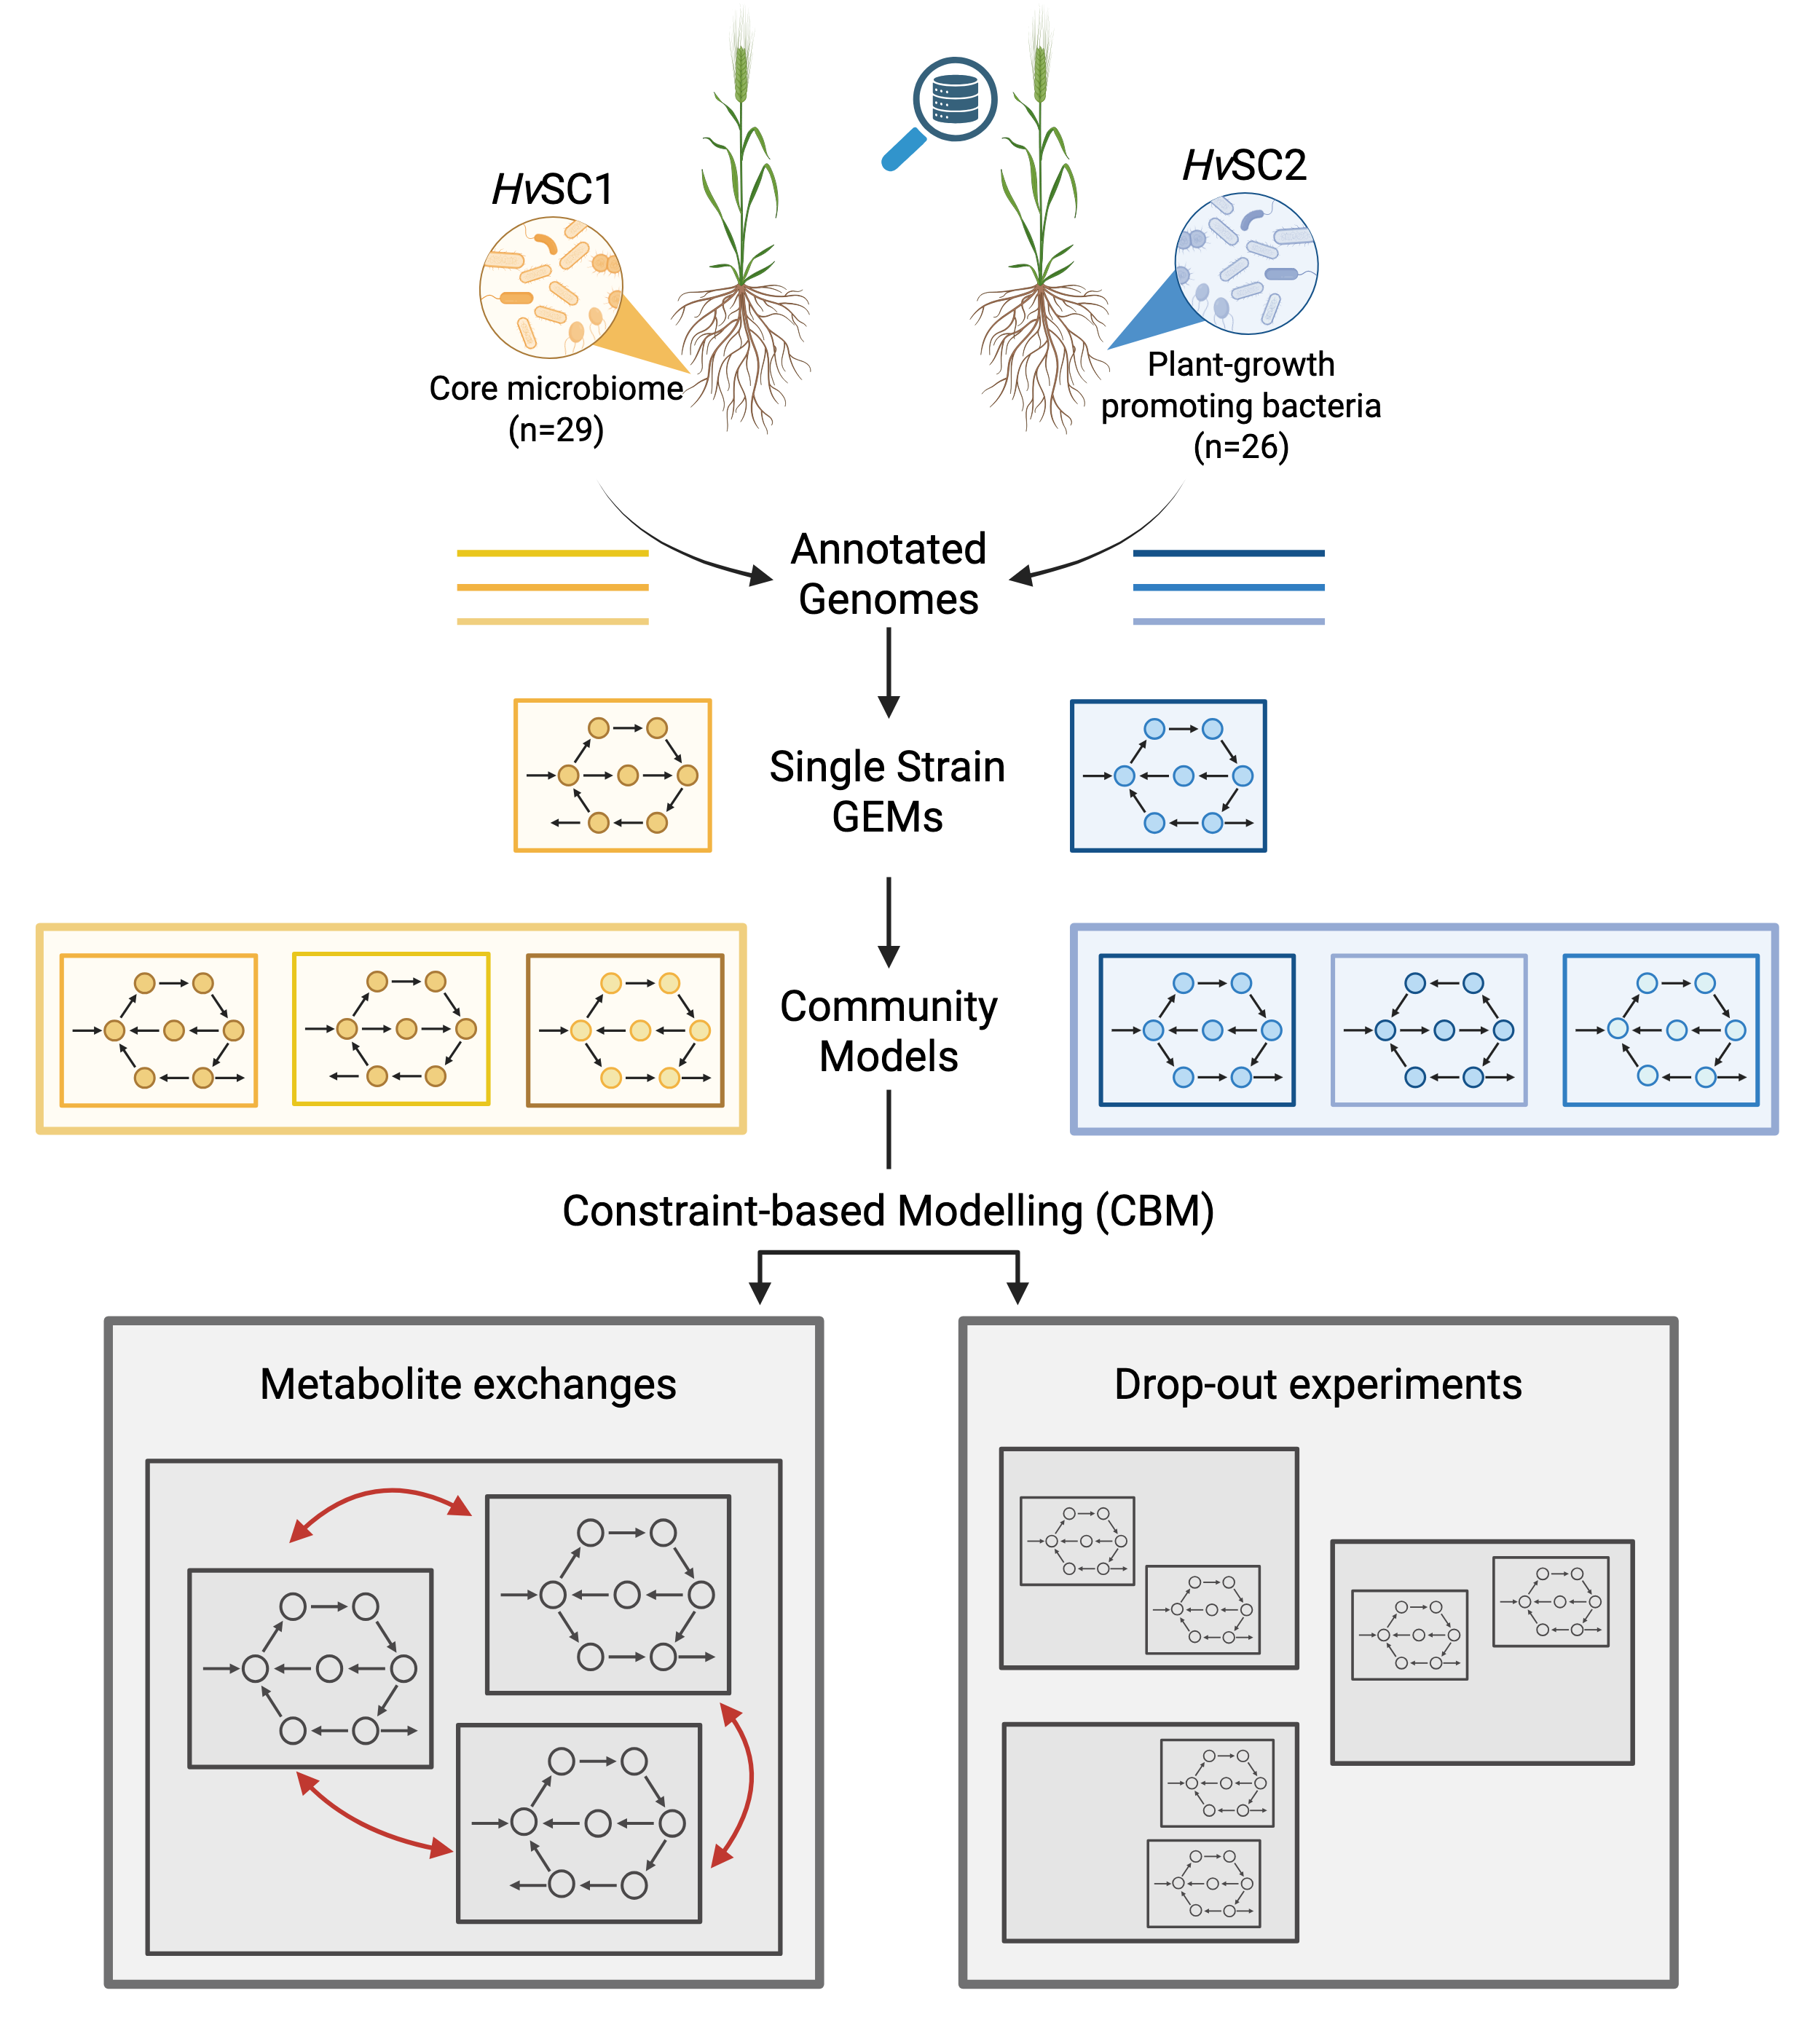
\includegraphics[width=1\textwidth]{fig/Graphical_abstract.png}
  \caption[Graphical abstract of the reconstruction and analysis workflow]{Graphical abstract of the reconstruction and analysis workflow. First, single strain genome-scale metabolic models (GEMs) were reconstructed from annotated genomes and assembled into community models. Using constraint-based modelling (CBM), metabolic behaviour, metabolite exchanges and drop-out experiments were evaluated. Created with BioRender.}
  \label{fig:graphical_abstract}
\end{figure}

The structure of this thesis follows the graphical abstract, as depicted in Figure \ref{fig:graphical_abstract}. 

\chapter{Background}
\section{Plant-microbe interactions}
The plant microbiome is made up of communities of microorganisms that inhabit the internal and external of plants, collectively forming a dynamic ecosystem that supports plant growth and pathogen protection. Rather than acting as completely isolated domains, the plant's two main spatial regions: the above-ground phyllosphere and the below-ground rhizosphere. Each encompasses both external (exosphere) and internal (endosphere) environments. The rhizosphere is the zone around plant roots, this zone is heavily enriched with organic materials from the plant and products from microbes and other organisms in this environment. 
As plants allocate up to 20\% of their photosynthetically derived carbon as exudates into the rhizosphere, the nutritional value of root released metabolites is high and therefore attracts soil microbes to the root (\cite{trivedi_plantmicrobiome_2020, hutsch_plant_2002}).
Members of a plant microbiota comprise beneficial, neutral, and pathogenic microorganisms, whose relative activity and balance determine whether microbiome function supports or undermines host health. Importantly, certain microbial traits manifest only within the context of a whole community and cannot be predicted from individual members alone (\cite{trivedi_plantmicrobiome_2020}).
\subsection{Metabolic interactions within microbial communities}
Metabolic interactions are driven by cross-feeding, antagonism and niche differentiation. A metabolic niche can be described as the set of genetically encoded metabolic functions that an organism needs to survive. Niche differentiation is the process by which competing species use the environment differently in a way that helps them to coexist. Antagonistic interactions are characterised by the secretion of specialised metabolites, which inhibit competitors or restrict their access to essential nutrients (\cite{wankhade_review_2025}). Cross-feeding describes interactions, where one microorganism consumes and utilises the metabolic byproducts or waste compounds secreted by another. Within such dynamics, certain community members can act as keystone species, playing an especially important role in stabilising their ecosystem. They exert a large number of (positive) interactions and their removal from the system significantly affects ecosystem productivity, nutrient cycling, and species richness (\cite{amit_top-down_2023, banerjee_keystone_2018}).
\subsection{Design and applications of synthetic communities}
Microbial communities compose a significant part of the rhizosphere. Elucidating the detailed mechanisms behind plant-microbe and microbe-microbe interactions however remains challenging, as the complex natural communities are difficult to analyse: Which members are actively participating in nutrient exchanges? Are all occurring rare species cultured? Which players perform key functions? (\cite{shayanthan_role_2022}). Some of these questions can be answered using Synthetic Communities (SynComs), which are composed of selected bacterial strains that together represent a simplified version of the microbiome while retaining functional traits. They are widely established as model systems for the analysis of performance, structure and stability of microbial communities. As the exact composition of the co-culture and the surrounding conditions are known, these defined systems reduce complexity while preserving key attributes of the natural community they represent (\cite{groskopf_synthetic_2014}). 
\subsubsection{Synthetic communities HvSC1 and HvSC2}
\cite{mahdi_low_2026} extensively cultured barley root endophytes across genetically distinct barley accessions, from which the SynComs investigated in this thesis were composed. Core strains were assembled to the core SynCom, HvSC1, its 29 members reflect taxonomic composition in the natural barley microbiome. The trait-prioritised SynCom, HvSC2, was assembled based on 26 strains previously associated with plant growth promotion or pathogen suppression and does not reflect natural co-occurrence (Fig. \ref{fig:taxonomic_distr}).
Experimental comparison of the two SynComs showed that microbial communities exhibiting little disruptive competition and low antagonism are favoured by host-associated environments. Beneficial microbiome function is promoted by balanced interspecies interactions rather than maximal antagonism and limited disruptive competition within a community. The conducted experiments contrasted the two communities in their antagonistic behaviour, stability and impact on plant growth: the core SynCom exhibited low antagonism and high stability, while guarding the host plant against fungal pathogens without reducing plant growth. Contrastingly, the trait-optimised SynCom was characterised by pervasive antagonism, competitive exclusion, community instability, and despite being composed of strains with predicted plant growth promoting traits, yielded loss of plant protective function and diminishing root growth (\cite{mahdi_low_2026}).

\begin{figure}[h]
  \centering
  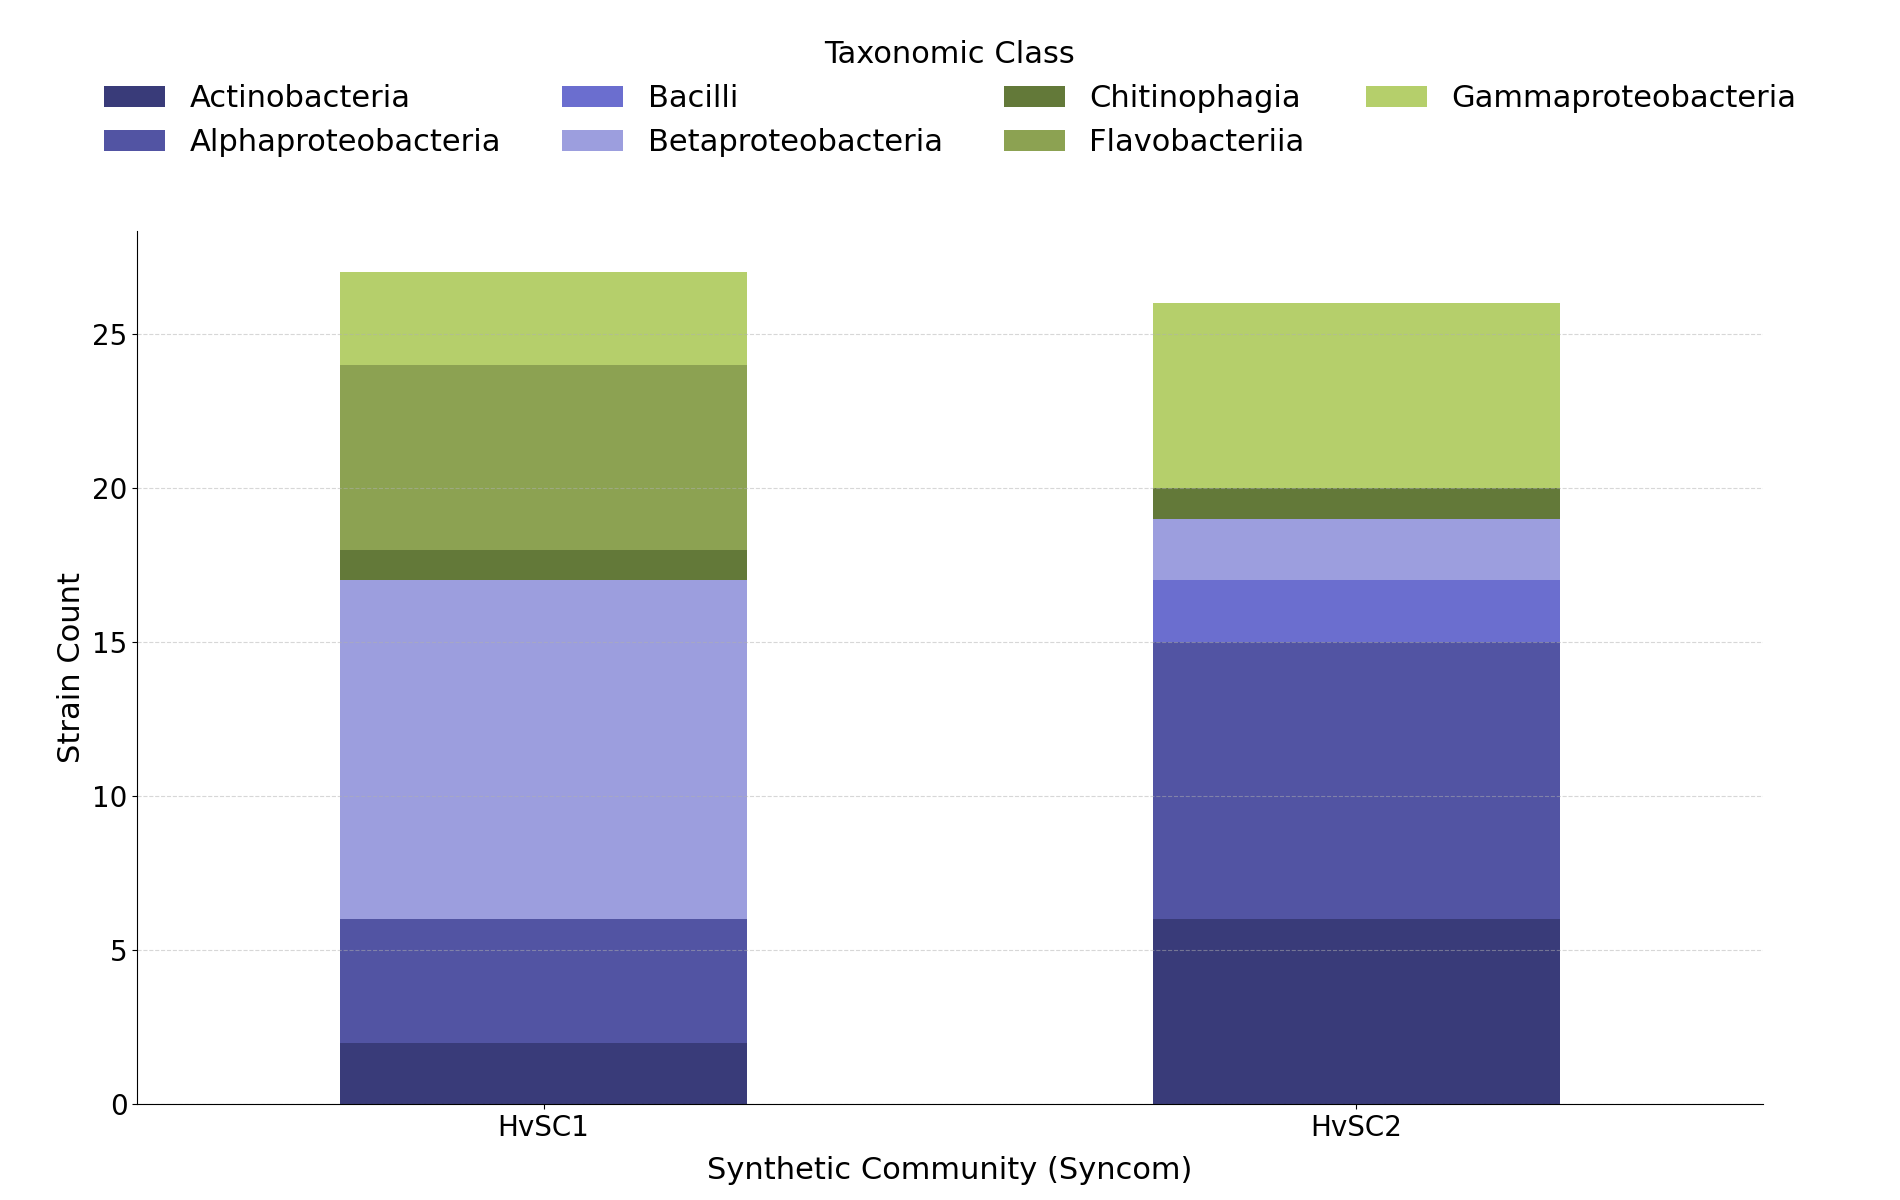
\includegraphics[width=1\textwidth]{fig/taxonomy_distr.png}
  \caption[Taxonomic class composition of the barley SynComs]{Taxonomic class composition of the barley SynComs. Stacked bar chart displaying the strain count across various taxonomic classes for two HvSC1 and HvSC2. Colors denote specific bacterial classes as indicated in the legend.}
  \label{fig:taxonomic_distr}
\end{figure}

\section{Genome-scale and constraint-based metabolic modelling}
\subsection{Metabolic network reconstruction}
Studying the complexity of metabolism in nature is often very challenging. Reconstructing metabolic networks into computational formats reduces complexity and can provide valuable insights into underlying structures.
Metabolic networks can be reconstructed in different approaches. Kinetic metabolic reconstruction is based on determining the appropriate reaction network followed by parameterising the rate laws with empirically based values, thereby allowing the simulation of dynamic behavior within a cell (\cite{cook_standardized_2026}). Stoichiometric based modelling is an alternative approach, which relies on metabolic steady states, meaning that the sum of all changes in metabolite concentrations $x$ over time is $0$ (\cite{orth_what_2010}). This approach requires less data and is therefore much more practical for genome-scale metabolic models and was employed in this thesis.
\\


Genome-scale metabolic models (GEMs) translate genomic information into mathematical formulations of metabolic networks. Such a metabolic network is represented as a stoichiometric matrix ($S$) of size $m  \times n $. Every row of this matrix represents one unique compound, every column a reaction, yielding $m$ metabolites and $n$ reactions. The entries of one column are the stoichiometric coefficients of the metabolite in this reaction. These are negative if the metabolite is consumed in the reaction and positive if this metabolite is produced in the reaction. A coefficient of zero means that the metabolite does not participate in the reaction. The flux through all the reactions of the system is represented by the vector $v$, with length $n$, the metabolite concentrations are represented by the vector $x$ with length $m$. Under the steady-state assumption, the system is described by $Sv = 0$. 
\\


One method to investigate these metabolic networks is constraint-based modelling (CBM), which can be used to analyse the solution space. A solution space is defined by all feasible phenotypic states, given a set of imposed constraints. These constraints arise from the relationship between the genotype of an organism, its environment and physico-chemical laws (\cite{bordbar_constraint-based_2014}). CBM scales to large-scale models, provides mechanistic understanding of molecular processes and does not require kinetic parameters, which are often hard to obtain. The strategy involves two major steps: first, constraining a biological system and then analysing the system to predict metabolic fluxes (Fig. \ref{fig:fbaworkflow}). 
\\


The constraining of a model usually modifies the metabolic reaction bounds and thereby defines the solution space. This can be achieved using various types of data, such as the uptake and secretion profiles of metabolites, or the expression levels of mRNA and proteins, to either setting the bounds of a reaction to zero if the corresponding protein is absent or scaling the bounds to the protein abundance. Once the model is parameterised, metabolic fluxes can be calculated. Flux balance analysis (FBA) is based on the assumption that a cell’s metabolism underlies an optimisation problem: a metabolic objective. This is either the minimisation or the maximisation of the flux of the objective function $Z = cTv$, with $c$ being a vector of weights indicating how much each reaction contributes to the objective function and $v$ being the flux vector. This objective can for example be set to growth (biomass synthesis reaction), the production of a certain compound, or energy generation (ATP production). FBA then utilises linear programming to obtain a flux distribution $v$ that optimised the objective function $Z$, subject to the steady-state constraint $Sv = 0$ and the imposed reaction bounds (the upper and lower bounds on $v$). Because there are more reactions than metabolites ($n$ > $m$), the system is underdetermined, meaning many flux distributions satisfy constraints. Among these, multiple different flux distributions can achieve the same optimal objective value, meaning the FBA solution itself is generally not unique. Flux variability analysis (FVA) addresses this by calculating, for each reaction, the minimum and maximum flux value consistent with (near-)optimal objective function values. Rather than evaluating flux ranges, parsimonious FBA (pFBA) narrows the solution space by applying an enzyme-efficiency constraint. It works in two steps: first it optimises the objective function and then minimises the flux through the model, thus minimizing the overall enzymatic and resource cost required to achieve that optimal state (\cite{lewis_constraining_2012, orth_what_2010}). 
Depending on the convergence of the algorithm, the solution status of such constraint-based problems varies. It indicates how accurate a solution might be. An overview of relevant return statuses can be found in Table \ref{tab:solution_statuses}. 

\begin{table}[htbp]
  \centering
  \caption{Solution statuses as returned by solver.}
  \label{tab:solution_statuses}
  \begin{tabular}{lp{10cm}}
    \hline
    \textbf{Return Status} & \textbf{Explanation according to (IBM CPLEX Optimizer for z/OS, 2021)} \\ \hline
    Optimal & The algorithm converged to a point satisfying all constraint tolerances and optimality conditions within specified bounds. Optimal solution is available. \\
    Numeric/ numeric best & Solution is available, but not proved optimal, due to numeric difficulties during optimization. \\
    Infeasible & Problem has been proven infeasible, there is no solution that satisfies all constraints simultaneously. \\ \hline
  \end{tabular}
\end{table}

\begin{figure}
	\centering
	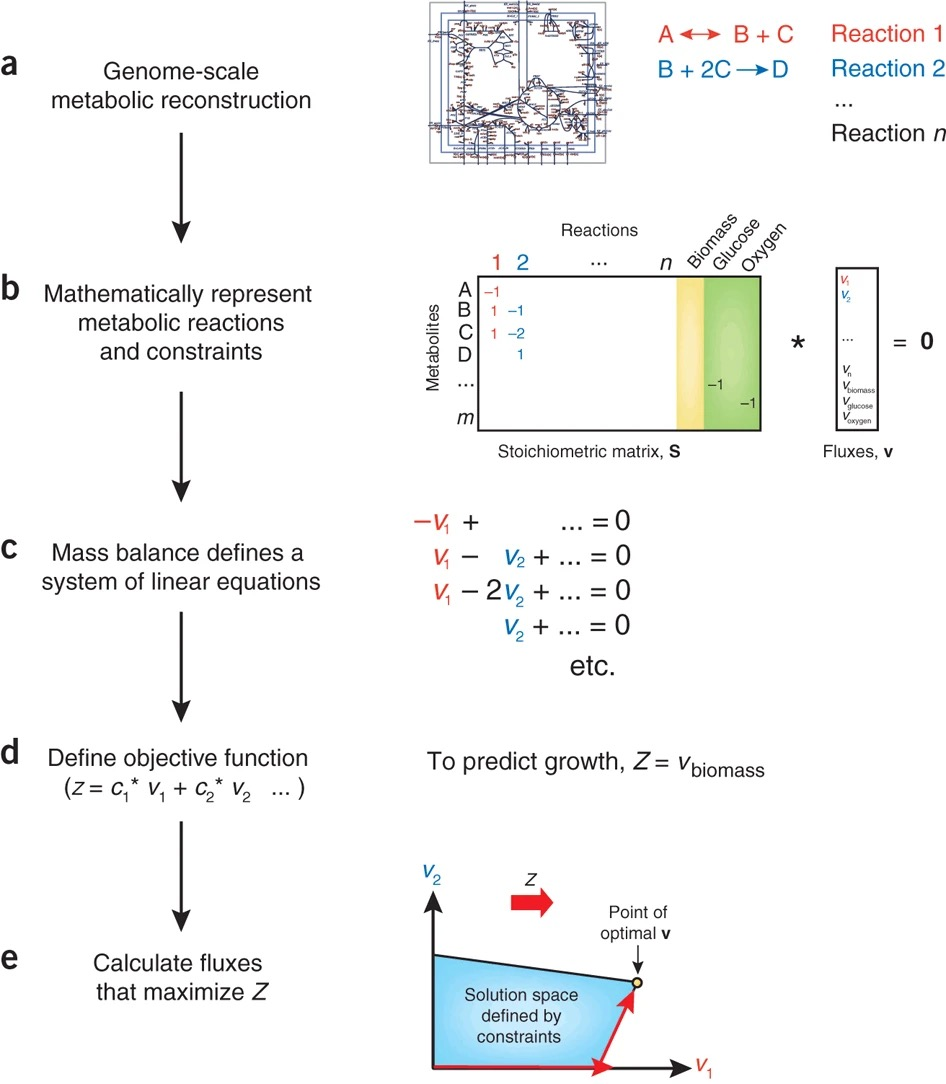
\includegraphics[width=0.9\linewidth]{fig/fba_workflow}
	\caption[Flowchart of constrained-based modelling]{Flowchart of constrained-based modelling. (a) Based on the genome of the organism, its metabolic network is reconstructed. (b) This network can be mathematically represented as a stoichiometric matrix S where each row stands for a metabolite and a column represents a reaction; each reactions has an associated flux value in the vector v. (c) Under the steady-state assumption, the matrix S and vector v form a system of linear equations. (d) Solving the equations required the definition of an objective function Z, which will be maximised during the optimisation step. (e) Linear programming is used to solve the linear equations and thereby find a flux distribution that maximises Z within the constrained solution space. Taken from \cite{orth_what_2010}.}
	\label{fig:fbaworkflow}
\end{figure}

\subsection{Reconstructing GEMs}
The basis for metabolic models forms an annotated genome, based on which, reactions and metabolites of the target organism can be inferred. Various tools have been developed to facilitate the reconstruction process. This process generally follows three steps: 
(i) Use databases and other prior knowledge to map the annotated genome to metabolic functions. 
(ii) Generate draft model. 
(iI) Curate the draft model.
A comprehensive review for tools employed in model reconstruction, quality control and curation can be found in \cite{tarzi_emerging_2024}.


Model reconstruction follows one of two approaches, or a combination of both. The first approach, known as 'top-down', begins with an existing network of biochemical reactions based on either genome-scale metabolic models that have already been reconstructed or a collection of all the reactions that have been identified in the organism of interest. This approach is typically faster and easier to automate, but lacks highly specific pathways and ideal accuracy. The second approach, called bottom-up, starts with known metabolic pathway stoichiometries and subsequently adds all known reactions and metabolites. This approach is much more time-consuming and labour-intensive, but it ensures very high accuracy and high quality models.
\\


A variety of tools can be employed to aid the model reconstruction. CarveMe (\cite{machado_fast_2018}) is one example of a tool that follows the top-down approach. Based on the entire bacterial metabolism in the BiGG database (\cite{king_bigg_2016}), it builds a universal model. All metabolites and reactions use BiGG identifiers. Additionally, each metabolite identifier ends with \_c, \_p or \_e according to its compartment (cytosol, periplasm or extracellular space).  According to the annotated genome of the target bacteria, the ‘carving’ process removes reactions and metabolites that are not predicted to occur in the organism. Depending on the gram-stain of the bacteria, it assigns a universal biomass function, which is a pseudoreaction that consists of all components required to produce new cell mass and the associated energy. CarveMe outputs the draft SBML model in .xml format that can be further analysed with COBRApy.

\subsubsection{Biomass in metabolic models}
\subsubsection{Biomass in metabolic models}
Fluxes are typically reported in $\text{mmol} \cdot \text{gDW}^{-1} \cdot \text{h}^{-1}$, where $\text{gDW}$ denotes gram dry weight of biomass and $\text{h}$ represents time in hours. The biomass metabolite within a model is a pseudo-metabolite that is usually defined by its precursors in the biomass reaction, rather than a single chemical compound. The molecular weight of the biomass of a metabolic model is typically normalised so that $1\text{ mmol}$ biomass corresponds to $1\text{ gDW}$, which is calculated by multiplying the coefficient of each metabolite of the biomass reaction with its molecular weight calculated from the formula, then dividing the overall sum of all the products by $1000$ \cite{lieven_memote_2020}. Therefore, the flux through the growth reaction can directly be interpreted as a growth rate in units of:
\[
\frac{\text{new biomass (gDW)}}{\text{existing biomass (gDW)} \cdot \text{h}}
\]
which yields $\text{h}^{-1}$ \cite{machado_fast_2018}. In other words: the growth rate $\mu$ is the instantaneous fractional rate at which biomass increases, i.e.\ $\frac{dX}{dt} = \mu \cdot X$, so at each timepoint, for a growth rate of $2\text{ h}^{-1}$, biomass is momentarily increasing at $2\text{ g}$ new biomass per $1\text{ g}$ existing biomass per hour. Integrating this relationship over an hour:
\[
X(t) = X_0 \cdot e^{\mu t}
\]
For $t = 1$ and $\mu = 2$:
\[
X(1) = X_0 \cdot e^{2} \approx X_0 \cdot 7.39
\]
\subsection{Quality assessment and curation of GEMs}
\cite{thiele_protocol_2010} defined the core principles of model reconstruction, network evaluation, refinement and curation, which remain central to the process today and guide the development of new automated approaches (Fig. \ref{fig:curation_workflow}). The quality of the models depends on the reconstruction approach taken and the quality of the underlying data. Quality is assessed and refined iteratively. Automatic algorithms evaluate model quality by detecting gaps and dead ends and by assessing consistency between the model and its annotation. A subsequent curation step then corrects and refines the model until it is consistent with experimental observations and fits community quality standards, to ensure an accurate representation of biological reality (Fig. \ref{fig:curation_workflow}).

\begin{figure}[h]
	\centering
	
\includegraphics[width=1\textwidth]{fig/curation_workflow_linear}
	\caption[Curation workflow]{Curation workflow. After draft model generation, several iterative steps are applied to refine, evaluate and improve the model. This schematic highlights key steps of the curation process established by \cite{thiele_protocol_2010})}
	\label{fig:curation_workflow}
\end{figure}


Manual quality control is very time and labour intensive and thus facilitated by various tools, amongst which are MACAW (\cite{moyer_macaw_2025}) and MEMOTE (\cite{lieven_memote_2020}). MEMOTE provides a comprehensive testing for consistency, annotation, biomass composition, energy metabolism, GPR rules, and network topology. Each test returns a score, all individual scores are then summed and weighted to an overall quality score. MACAW focuses on structural and functional checks, such as identifying duplicated, dead ends, and thermodynamically infeasible loops. The output of these tools and proposed steps in the \cite{thiele_protocol_2010} protocol guide the curation process. 
\subsection{Tools for community modelling}
Microbial communities are a fundamental unit in complex ecosystems, and deciphering their functionality, structure and other properties is of high interest across different disciplines. Thus many methods and tools have been developed to study microbial interactions. To analyse such interactions on a metabolic level, tools like COMMA (\cite{mirzaei_gem-based_2024}), MICOM (\cite{diener_micom_2020}), PyCoMo (\cite{predl_pycomo_2024}) or ReMIND (\cite{oftadeh_constraint-based_2024}) build community from taxon models following the steady-state approach. The tools differ in their required taxonomic information, analysis of microbial interactions, formulation of the objective function, as well as compartmentalisation strategy and are comprehensively reviewed in (\cite{tarzi_emerging_2024}). 
\subsubsection{MICOM} \label{sec:MICOM}
MICOM combines individual strain models into a unified community model with a shared medium compartment. Specifically, the extracellular compartment of every single-taxon input model is connected via an exchange reaction to a shared pool (\_m) through which community members interact. Exchange reactions from the shared medium \_m compartment to an individual's extracellular compartment \_e are either uptakes or secretions, depending on the direction of reaction. 

The community growth rate $\mu_c$ is calculated as the weighted sum of the individual growth rates $\mu_i$ of each organism $i$ and its relative abundances $a_i$. MICOM offers two different optimisation strategies: \texttt{optimise()}, which is simply a (p)FBA solution for the whole community, and \texttt{cooperative\_tradeoff()}, which optimises the objective function under user-provided abundance data and a trade-off approach between community and individual growth rate maximisation. This prevents the exclusion of strains known to be abundant for the sake of maximising the community growth rate. In practice, MICOM first maximises $\mu_c$, yielding the maximum community growth rate $\mu_c^{max}$. Then, the chosen trade-off $\alpha \in [0,1]$ sets the minimum fraction of $\mu_c^{max}$ that has to be achieved. Setting the trade-off to 0 optimises for individual growth, whereas a trade-off of 1 solves for maximal community growth. This sets up the quadratic minimisation problem following L2 regularisation: 

\begin{equation}
	\begin{aligned}
		&\text{minimise} & &\sum_{i} \mu_i^2 \\
		&\text{s.t.}     & &\mu_c \geq \alpha \mu_c^{\max} \\
		&                & &\text{and community constraints}
	\end{aligned}
\end{equation}
	
	
It favors balanced solutions with more equally distributed growth rate across community members, which is shown to yield more realistic growth rates (\cite{diener_micom_2020}). 


\chapter{Methods}

For reconstructing, simulating and analysing the two SynComs and their members \textit{in silico}, I used Python together with COnstraints-Based Reconstruction and Analysis (COBRA) methods, implemented in the COBRApy package (\cite{ebrahim_cobrapy_2013}). Cplex 22.1.1 (\cite{noauthor_ibm_2022}) was the solver for all performed simulations. The complete code for model reconstruction, evaluation and analysis is available in the supplementary folder provided with this thesis.
\section{Generation of Draft Models}
All my analyses build on the genome-scale metabolic models of the 50 individual community members. A detailed list of all members, their taxonomic information and Gram staining classification can be found in the appendix (Table \ref{tab:syncom_isolates}). Each strain has a three- or four-digit ID, which is how it will be referred to in this thesis. Genome assemblies were annotated using Bakta (\cite{schwengers_bakta_2021}). Bakta performs rapid and standardised annotation of bacterial genomes using a combination of alignment-free protein sequence finders, highly curated databases like UniProt, and hidden Markov models for structural features. Based on these annotated genomes, I used the Gram-specific workflow in CarveMe (\cite{machado_fast_2018}) to generate a draft model for each community member. 
\section{Evaluation and Curation of Draft Models}
The quality of the draft models was assessed using MEMOTE (\cite{lieven_memote_2020}). Based on these reports, the models were curated. This involved several steps: 
\begin{enumerate}
    \item Metabolite and reaction information were automatically overwritten with BiGG information to obtain consistent formulas and charge states. Imbalanced reactions were systematically identified and updated with standard BiGG stoichiometric definitions.
    \item Manual charge and mass balancing of remaining imbalanced reactions from step (I): While the initial curation script was able to balance most of the reactions, I manually corrected 76 reactions, balancing all masses. The remaining charge imbalances, a minority of 82 reactions which mostly stem from pH-dependent protonation states, were not further corrected. 
    \item Metabolite duplicate removal of metabolites flagged in the MEMOTE report. 
    \item MACAW (\cite{moyer_macaw_2025}) was used as an additional tool for analysing reaction duplicates and reversibility of reactions including diphosphates. MACAW classifies duplicates into exact, directional, coefficient, and redox categories, which allows for easier correction later on. This curation step was also split in an automated and manual part, the first focusing on exact and directional duplicates, while the latter corrected all remaining reactions. Duplicate reactions featuring different Gene-Protein-Reaction (GPR) associations were resolved systematically: if a GPR was present in only one of the duplicate reactions, the reaction lacking the GPR was deleted, whereas if neither reaction was associated with a GPR, the version with lower prevalence in the BiGG database was removed. Conversely, duplicate reactions that differed solely in their coefficients, redox pairs, or reversibility (and consequently maintained different GPRs) were left unchanged. While these duplicates remain within the final model, they are biologically correct as they represent functionally different variants, such as isoenzymes. 
    \item Twenty metabolites were flagged as dead-end, orphaned, and/or unconnected in the MEMOTE report of models after step 4. Their correction involved deleting previously undetected duplicate metabolites and adding missing pathway-connecting reactions. The peptidoglycan synthesis pathway was also adjusted to ensure biological correctness. The pentapeptide intermediates contain a \textit{meso}-A2pm residue in Gram-negative bacteria and \textit{Bacillus} species, whereas in other Gram-positive models, they contain a lysine residue (\cite{bouhss_biosynthesis_2008}). Therefore, the pentapeptide \texttt{uaagmda}, which contains a \textit{meso}-A2pm residue, was replaced with \texttt{uaaGLa}, which contains a lysine residue. Because the precursors needed to replace the other pentapeptides were unknown, only \texttt{uaagmda} was replaced, and the other intermediates with \textit{meso}-A2pm residues were kept.
    \item Assessing growth function of all models. CarveMe modifies the biomass reactions for Gram-positive and Gram-negative bacteria, as they differ in their membrane and cell wall compositions. Production of all required components may not be feasible in all models, because CarveMe predicts an organism's uptake and secretion capabilities based on phylogeny and thus may lack specificity on the strain level. To ensure growth of all the curated models on complete medium (i.e., a nutrient-rich medium that allows for all possible exchanges), the synthesis of all biomass educts was evaluated individually for each biomass educt. This was achieved by setting the demand function, i.e., the irreversible reaction consuming the metabolite, as the objective function for an FBA. There was only one model (895) that was unable to produce all biomass educts: here the synthesis of menaquinol 8 (\texttt{mql8}) failed. Literature states that menaquinone reactions and hence menaquinol synthesis are highly conserved in all Gram-positive and facultative anaerobic Gram-negative bacteria (\cite{boersch_menaquinone_2018}). Strain 895 is one of many aerobe, Gram-negative bacteria in the communities, while all others were able to produce menaquinol, this one was not and should therefore use ubiquinol instead (\cite{pelosi_ubiquinone_2019}). \texttt{Mql8\_c} was replaced with \texttt{q8h2\_c} in the growth reaction and the synthesis pathway for ubiquinol was completed.
\end{enumerate}

To quantify the improvements made in the curation process, after performing all curation steps, I reevaluated the quality of the curated models with MEMOTE. 
\section{Creation of complete apoplastic medium}
To mirror the communities’ natural environment as closely as possible, I used metabolomics data from \cite{saake_ergosterol-induced_2025} to reconstruct the medium based on the metabolic composition of the apoplastic fluid in the barley rhizosphere. Compound names were first translated into BiGG IDs and then into the corresponding exchange reactions. The upper bounds of all reactions were constrained based on abundance: the most abundant metabolite was assigned an upper bound of 1000 mmol/(gDw *h) and the other upper bounds were scaled accordingly. Next, the metabolites were categorised according to their flux into groups with upper bounds of 0.1, 10, 100, 500 and 1000 (all in units of mmol/(gDw *h)). Based on community standards of unrestricted secretions, the lower bounds got constrained to -1000 mmol/(gDw *h).This tiered medium, containing 58 compounds, is referred to as the base apoplastic medium. 
The base apoplastic medium was then completed individually for each community, using MICOM’s \texttt{complete\_medium()} function, while minimising the number of medium components. The minimum community growth rate was set to 1, and the minimum individual growth rate was set to 1/n (where n is the size of the community). The two completed media were then merged to create a final completed medium containing a total of 52 metabolites. If a metabolite was present in both media, the final medium was given the higher of the two fluxes. To maintain consistency, the fluxes of the added components were adjusted to fit the tiered medium. For more detailed steps, refer to Supplementary Figure \ref{fig:medium_completion}. 
The composition of the final medium can be found in Table \ref{tab:apoplastic_fluid_medium} (compound categories) and Table \ref{tab:medium_composition_2} (detailed compound list). Unless indicated otherwise, this medium was used for all simulations and subsequent analyses. 

\begin{table}[htbp]
  \centering
  \caption{Completed apoplastic fluid medium composition in metabolite classes.}
  \label{tab:apoplastic_fluid_medium}
  \begin{tabular}{lc}
    \hline
    \textbf{Category} & \textbf{Number of components} \\ \hline
    Organic Acids \& Carboxylates & 7 \\
    Carbohydrates, Sugars \& Derivatives & 9 \\
    Amino Acids, Peptides \& Polyamine & 16 \\
    Inorganic Compounds, Ions \& Gases & 19 \\
    Fatty Acids, Lipids \& Steroids & 1 \\ \hline
  \end{tabular}
\end{table}

\section{Construction and simulation of community models} \label{sec:Construction and simulation of community models}
The SynComs established by \cite{mahdi_low_2026} were reconstructed using the Python package MICOM (\cite{diener_micom_2020}). Using the curated models and a taxonomy file as input for the ‘Community()’ function, the community models HvSC1 and HvSC2 were reconstructed. Within a community, the members were all equally abundant.
The objective of each community is set to maximal community growth ($\alpha$ = 1.0) while minimising differences between individual growth rates (L2 regularisation) and minimising the sum of fluxes (pFBA). To stay consistent with the community growth rate all reported individual growth rates are scaled by their abundance (which is 1/community size). 
\subsection{Evaluating interactions within community models}
\subsubsection{Niche overlap}
Niche overlap was quantified by two measures: Metabolic Resource Overlap (MRO score) and metabolite co-consumption. The MRO score (see Equation \ref{eq:MRO}) provides an upper bound on the overall degree of resource competition by comparing the set of minimal metabolic requirements required for growth $M_i$ of each community member $i$ within an interacting community of size $N$ (\cite{zelezniak_metabolic_2015}). It ranges from 0.0 (no overlap) to 1.0 (identical resource usage). Metabolite co-consumption describes the number of metabolites that are taken up by both strains within a strain pair of a community (\cite{diener_micom_2020}).
\begin{equation}
	MRO = \frac{n \displaystyle\sum_{i, j \mid i \neq j} |M_i \cap M_j|}{C(n, 2) \displaystyle\sum_{i=0}^{N} |M_i|}
	\label{eq:MRO}
\end{equation}
\subsubsection{Cross-feeding}
Metabolic interactions were evaluated using three metrics: the Metabolic Interaction Potential (MIP) score (Equation \ref{eq:MIP}), the flux-based Metabolic Interaction Potential (fMIP) score (Equation \ref{eq:fMIP}), and pairwise cross-feeding assessment. The MIP score measures the reduction in growth-essential compound requirements when species cross-feed by comparing the minimal number of components required for the growth of all members in a non-interacting ($M$) and interacting community ($I$). In contrast, the fMIP score quantifies the proportion of total community flux derived directly from interspecies metabolic exchanges.
\begin{equation}
	MIP = M - I
	\label{eq:MIP}
\end{equation}
\begin{equation}
  fMIP = \frac{\sum flux_{all} - \sum flux_{medium}}{\sum flux_{all}}
  \label{eq:fMIP}
\end{equation}
To identify potential cross-feeding interactions, each combination of strains was assessed for their exchange reactions by comparing the uptakes and secretions individually. Further, the total amount of uptaken and secreted metabolites was compared per taxon, yielding an overview about the most active interaction partners.

\subsubsection{Symmetry of interactions}
Metabolic interactions between pairs of community members can be symmetric in the number of exchanged metabolites or in the magnitude of interactions (sum of fluxes for one pairwise interaction). An interaction is said to be symmetric, if both partners provide the same amount of metabolites (or the same total sum of fluxes) in a pairwise interaction, and asymmetric, if one partner is the primary provider either in number of exchanged metabolites or flux magnitude.

\subsection{Drop-out and drop-in experiments}
Community drop-out experiments were performed in a high-performance computing environment. Following the same procedure as for the complete communities (see Section \ref{sec:Construction and simulation of community models}), each of the 27 (HvSC1) and 26 (HvSC2) drop-out communities were built, by omitting one strain at a time. Community and individual growth rates were compared across drop-outs.

\chapter{Results}

All models and the following analyses are provided as .xml files and Jupyter notebooks respectively in the supplementary folder.
\section{Reconstruction of metabolic models and community model creation}
The basis for all my analysis form the reconstructed metabolic models of the two SynComs. Therefore, my first research question that investigates the models in terms of their compliance to community standards is essential. 

Of the total 52 individual strains cultured in vitro, only 50 assembled genomes were available. The reconstruction process yielded 50 models containing 2,559 reactions and 1,676 metabolites on average, distributed across three compartments (cytosol, periplasm and extracellular space).
Evaluation of the MEMOTE reports revealed 8 mass and 961 charge imbalanced reactions (see Table~\ref{tab:curation_imbalances}). MEMOTE differentiates between these imbalances, however a reaction can be flagged as both mass- and charge imbalanced at the same time and will therefore be reported twice. Mass imbalances occur due to different protonation states of metabolites, causing an uneven number of protons on the reactant and product side or are a result of the incomplete resolution of placeholders in compound formulas ($X$ and $R$). The latter explains also why there are more mass imbalances after the automated curation step, which nevertheless decreased the number of charge imbalanced reactions by more than half. Charge imbalances are mainly caused by differing amounts of protons in the chemical formula and the charge state of a metabolite. All in all, through manual curation I achieved stoichiometric consistent models with no mass imbalances and only 82 charge imbalanced reactions (see Table~\ref{tab:curation_imbalances}).

\begin{table}[H]
  \centering
  \caption{Mass and charge imbalances across draft, automated BiGG overwrite, and curated models.}
  \label{tab:curation_imbalances}
  \begin{tabularx}{\linewidth}{Xccc}
    \hline
    \textbf{Metric} & \textbf{Draft models} & \textbf{Post automated BiGG overwrite} & \textbf{Curated models} \\ \hline
    Sum of all mass imbalances across all models & 190 & 2105 & 0 \\
    Total distinct mass imbalances across all models & 8 & 124 & 0 \\
    Sum of all charge imbalances across all models & 22512 & 9622 & 807 \\
    Total distinct charge imbalances across all models & 961 & 453 & 82 \\ \hline
  \end{tabularx}
\end{table}

Further curation steps focused on dead-ends, blocked reactions and removing the duplicates detected by MEMOTE and MACAW. MEMOTE flagged 45 average blocked reactions per model, which are defined as reactions that are not able to carry flux, indicating network gaps. MACAW highlighted further duplicates, which were resolved. Due to the substantial number of blocked reactions and energy-generating cycles and the considerable amount of time required to resolve them, their investigation was beyond the scope of this thesis.

\begin{table}[H]
  \centering
  \caption{Comparison of average model metrics before and after curation}
  \label{tab:average_model_metrics}
  \begin{tabularx}{\linewidth}{Xccc}
    \hline
    \textbf{Metric} & \textbf{Draft models} & \textbf{Curated models} \\ \hline
    Number of reactions per model & 2558.64 & 2536.12 \\
    Number of metabolites per model & 1675.50 & 1671.24 \\
    MEMOTE consistency score all models & 0.58 & 0.93 \\
    MEMOTE final score all models & 0.73 & 0.86 \\ \hline
  \end{tabularx}
\end{table}

Compared to the draft models, the average final MEMOTE score increased by 13\%, and the consistency score improved 35\% (see Table \ref{tab:average_model_metrics}). Unbounded fluxes in the medium and annotation gaps caused the remaining inconsistencies and imperfect scores. Overall the curation efforts clearly improved the structural and metabolic consistency of the models, establishing a robust, standardised foundation for subsequent analyses.
\\


Upon finishing the curation process, the SynComs were assembled using the tool MICOM \cite{diener_micom_2020}. The resulting core community contains $27$ members which accumulate $46{,}468$ metabolites and $70{,}762$ reactions. The resulting trait-optimised community is composed of $26$ members, totaling to $43{,}490$ metabolites and $65{,}177$ reactions. This large number of objects is due to MICOM's compartmentalisation strategy, where each metabolite and reaction is specific to the compartment and strain it is built in. For example, intracellular glucose is formatted as \texttt{glc\_\_D\_c\_\_\{strain\_id\}} instead of \texttt{glc\_\_D\_c}. Condensing the reactions and metabolites by compartment and strain, HvSC1 contains $5{,}293$ unique reactions and $1{,}622$ unique metabolites, whereas HvSC2 contains $5{,}455$ reactions and $1{,}667$ metabolites.


\section{Choice of the optimisation method}
To obtain the communities’ metabolic fluxes, which are the basis for all subsequent analysis steps, I optimised the models for community growth. Furthermore, testing growth is one way to evaluate model quality, directly addressing my first research question. During my simulations, I tested different optimisation methods that are included within the MICOM package (Section \ref{sec:MICOM}). This investigation was primarily motivated by improbable results observed in one experiment: when applying \texttt{cooperative\_tradeoff()}, across all trade-off values $\alpha$, artificially blocking sugar exchanges within the community resulted in higher overall community growth rates compared to scenarios where sugar secretion was allowed. This outcome does not align with the basic assumptions of constraint-based modelling, as removal of a constraint (block of the secretion) expands the feasible flux space, which can not have a lower global optimum than a constrained subset. Therefore, the community growth rate should be equal or lower for additional constraints, never higher. This error did not occur when using the standard \texttt{optimise()} objective function. 
\\


The discrepancy led to a more detailed systematic evaluation and comparison of MICOM's underlying optimisation strategies. The \texttt{optimise()} method consistently yields the highest total community growth rate across all tested methods. However, it also results in the highest number of non-growing strains within the community. Furthermore, under this strategy I observed non-growing strains which still carried active metabolic fluxes. Biologically this result is unrealistic as these strains are used as passive, extracellular extensions of active strains rather than distinct living organisms. This underlines the need for further regularisation of growth rates, as done with the trade-off strategy. 
To mitigate these problems caused by MICOM’s optimisation function, I introduced a custom trade-off function, which is based on MICOM's \texttt{cooperative\_tradeoff()}, see Section \ref{sec:MICOM}, but bypasses the crossover strategy and accepts non-optimal, yet numeric results (see Table \ref{tab:solution_statuses}). 


\section{Comparison of community and individual growth rates}
The predicted growth of a model is one indicator of its quality. Therefore, to answer the first research question, I assessed the individual strain and the community growth in their native environment: the barley apoplastic fluid. None of the models showed growth in monoculture on the apoplastic medium, highlighting the significance of community interactions in enabling growth. 
\\


In the community context, the core community exhibits higher growth rates ($\mu_{c1} = 7.534 \text{h}^{-1}$ vs. $\mu_{c2} = 5.945 \text{h}^{-1}$), as well as higher growth rates among its members. Median individual growth rates are higher in HvSC1 ($\mu_{i,\text{median}} = 0.236\,\text{h}^{-1}$) than in HvSC2 ($\mu_{i,\text{median}} = 0.212\,\text{h}^{-1}$). While this difference may seem minor, the clustering of the individual values around this median differs noticeably: HvSC1 growth rates are far more tightly clustered around the median (IQR: 0.04), whereas HvSC2 spanned a much wider range (IQR 0.09) (Fig.~\ref{fig:growth_comparison}). 
The three taxa present in both communities consistently grow stronger in the core community (see green coloured strains in Fig.~\ref{fig:growth_comparison}), which shows that the difference in community growth rate can not only be attributed to differences in taxa composition but also community interactions. This pattern is underlined by taxa with small growth rates. Only one strain in HvSC1, namely 1124, grows less than $0.1\,\text{h}^{-1}$, compared to four taxa in HvSC2. Growth in the core community is both higher on average and generally more evenly distributed, with smaller differences in individual growth rates compared to the trait-optimised community.

\begin{figure}[H]
  \centering
  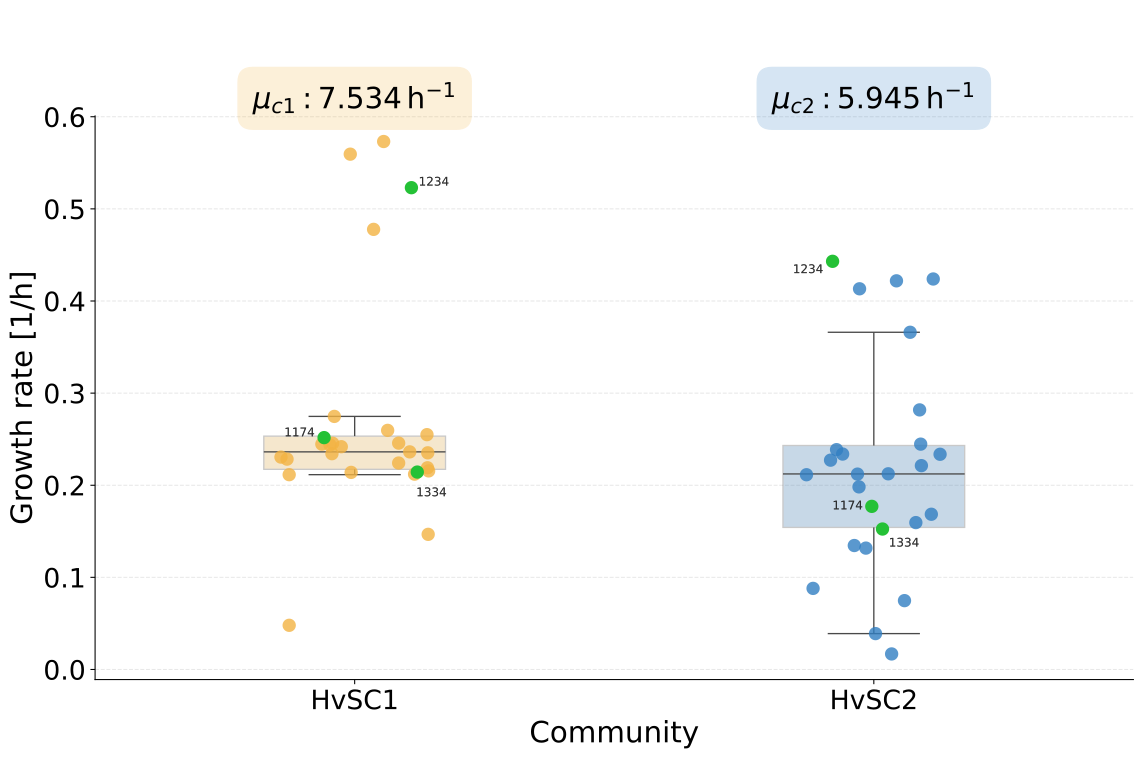
\includegraphics[width=1\textwidth]{fig/Individual_growthrates_boxplot_l2pfba_labels.png}
  \caption[Comparison of individual taxon growth rates by community on completed apoplastic fluid medium]{Comparison of individual taxon growth rates by community on completed apoplastic fluid medium. Community is indicated by colour: HvSC1 (yellow) and HvSC2 (blue). Green strains occur in both communities. HvSC1 shows higher community growth $\mu_c$ as well as higher average individual growth rates $\mu_i$, which are also more centered around the median, compared to HvSC2.}
  \label{fig:growth_comparison}
\end{figure}

\section{Metabolic profiles of each community}
To understand the metabolic requirements of each community, their internal niche overlap as well as the cross-feeding within a community, and thus answer the second research question, I analysed the uptake and secretion profiles of each community. These I obtained from growth simulations on the completed apoplastic fluid medium. Both communities take up 42 metabolites from the apoplastic medium, of which 40 are shared between the communities. These include amino acids, sugars as well as inorganic ions and provide the basis for growth. HvSC1 exclusively takes up UDP-N-acetyl-D-glucosamine, and HvSC2 exclusively utilises succinate. Beyond these medium-derived uptakes, the majority of uptake reactions (488 in HvSC1 and 504 in HvSC2) correspond to metabolites not present in the medium and thus are cross-fed metabolites between community members.
\subsection{Niche overlap}
Based on the collective uptakes of each community, I assessed their metabolic niche. The core community exhibits a larger niche overlap compared to the trait-optimised community, as shown by the higher MRO score, increased co-consumption (Fig. \ref{fig:combinednumbercoconsumptionsheatmap}) and smaller number of metabolites taken up only by a small fraction of the community (Table \ref{tab:metabolic_profiles}). This is in line with the larger number of metabolites exchanged in the native community, showing that the nutritional requirements within the community overlap more, reflecting their common co-occurrence, while the other community's nutritional requirements are more diverse.
As the range of possible uptakes from the medium was already limited due to the medium composition, no other clear metabolic niches became apparent. Other differences in metabolic profiles are therefore primarily caused by differences in cross-feeding behaviour.

\begin{table}[H]
  \centering
  \caption{Comparison of community interaction metrics for HvSC1 and HvSC2.}
  \label{tab:metabolic_profiles}
  \begin{tabularx}{\linewidth}{Xccc}
    \hline
    \textbf{Metric} & \textbf{HvSC1} & \textbf{HvSC2} \\ \hline
    Average number of co-consumed metabolites for each taxon pair & 43 & 39 \\
    MRO score & 0.512 & 0.501 \\
    MIP & 0.911 & 0.914 \\
    fMIP & 0.376 & 0.469 \\
    Average number of exchanged metabolites for each taxon pair & 15.060 (SD 11.003) & 12.378 (SD 8.414) \\
    Average sum of fluxes per pair & 1.974 (SD 2.186) & 3.846 (SD 3.561) \\
    Number of metabolites taken up by five members or less & 224 & 275 \\ \hline
  \end{tabularx}
\end{table}

\subsection{Metabolic interactions within the communities}
\subsubsection{Metrics in pairwise interactions}
Both communities show extensive amounts of cross-feeding, covering more than 90\% of their required metabolite range through community interactions (MIP score). However, while the potential range of shared metabolites (MIP) is nearly identical between the two communities, the flux volume through these pathways (fMIP) differs. Community interactions account for almost half of the total uptake fluxes in the trait-optimised community, whereas the more than 60\% of the core communities' uptakes stem from medium uptakes. Thus, while both communities share a similar diversity of cross-fed compounds, HvSC2 routes a larger magnitude of its overall metabolic flux through these community exchanges (Table \ref{tab:metabolic_profiles}).

An evaluation of pair-wise interactions within the communities underlines this result: The total sum of exchanged fluxes is higher in HvSC2 than in HvSC1 (Fig. \ref{fig:absolut_metaboliteinteractions}A, B). Strain 709 stands out, as it shares relatively high exchange fluxes with almost all members of HvSC2. This is not mirrored in the diversity of its exchanges: the total number of distinct exchanges is generally lower across HvSC2. Conversely, HvSC1 relies on a broader range of smaller exchanges, with Strains 892 and 1334 exchanging numerous different metabolites with fellow community members (Fig. \ref{fig:absolut_metaboliteinteractions}C).
\\


Importantly, interaction frequency does not directly scale with flux volume. High cumulative flux in the communities stems either from many minor exchanges or a few high-magnitude interactions. Overall, HvSC1 exchanges more metabolites distributed across smaller fluxes and wider spanned across the community. HvSC2 features less exchanged metabolites but a substantially higher flux volumes per interaction.
\begin{figure}[H]
	\centering
	
\includegraphics[width=1\linewidth]{fig/Combined_nex_sumflux_heatmap}
	\caption[Pairwise metabolic interaction in absolute numbers]{Pairwise metabolic interaction in absolute numbers. The heatmaps show pairwise cross-feeding interactions in scope of  magnitude (A, B) and number of exchanged metabolites (C, D). While HvSC1 is generally exchanges more metabolites, HvSC2 exhibits higher fluxes in its exchanges.}
	\label{fig:absolut_metaboliteinteractions}
\end{figure}


\subsubsection{Symmetry in metabolic interactions}
HvSC1 exhibits greater network connectedness, averaging more exchanged metabolites per strain pair, but with lower and more symmetric exchange fluxes. Symmetric exchange fluxes mean, that in a pairwise interaction assessment partner X provides the same flux amount as partner Y.  Based on flux magnitudes, no clear donor-only or recipient-only strains can be identified in HvSC1 (Fig. \ref{fig:balance_metabolicexchanges}A). In contrast, exchange fluxes in HvSC2 are heavily asymmetric: Strain 709 dominates flux magnitude as a major provider of amino acids and ethanol, while strains 1101 and 939 stand out as key providers of nucleotides, thiamine, and ammonium (Fig. \ref{fig:balance_metabolicexchanges}B). The symmetry in the number of exchanged metabolites follows the opposite pattern between the communities. In HvSC1 the group of strains 100, 1167, 1391, 163, 230, and 2774 stands out as wide-range providers. Notably, strains 1334 and 892 cross-feed with all community members in highly diverse metabolite exchanges (Fig. \ref{fig:balance_metabolicexchanges}D). HvSC2 is overall more symmetric, and therefore more balanced in the diversity of its exchanges, even though its flux magnitudes are heavily donor-driven.
This contrast highlights that the core community is more metabolically interdependent and reciprocal in flux exchange, relying on a distributed network of strains rather than a single donor strain.

\begin{figure}[H]
	\centering
	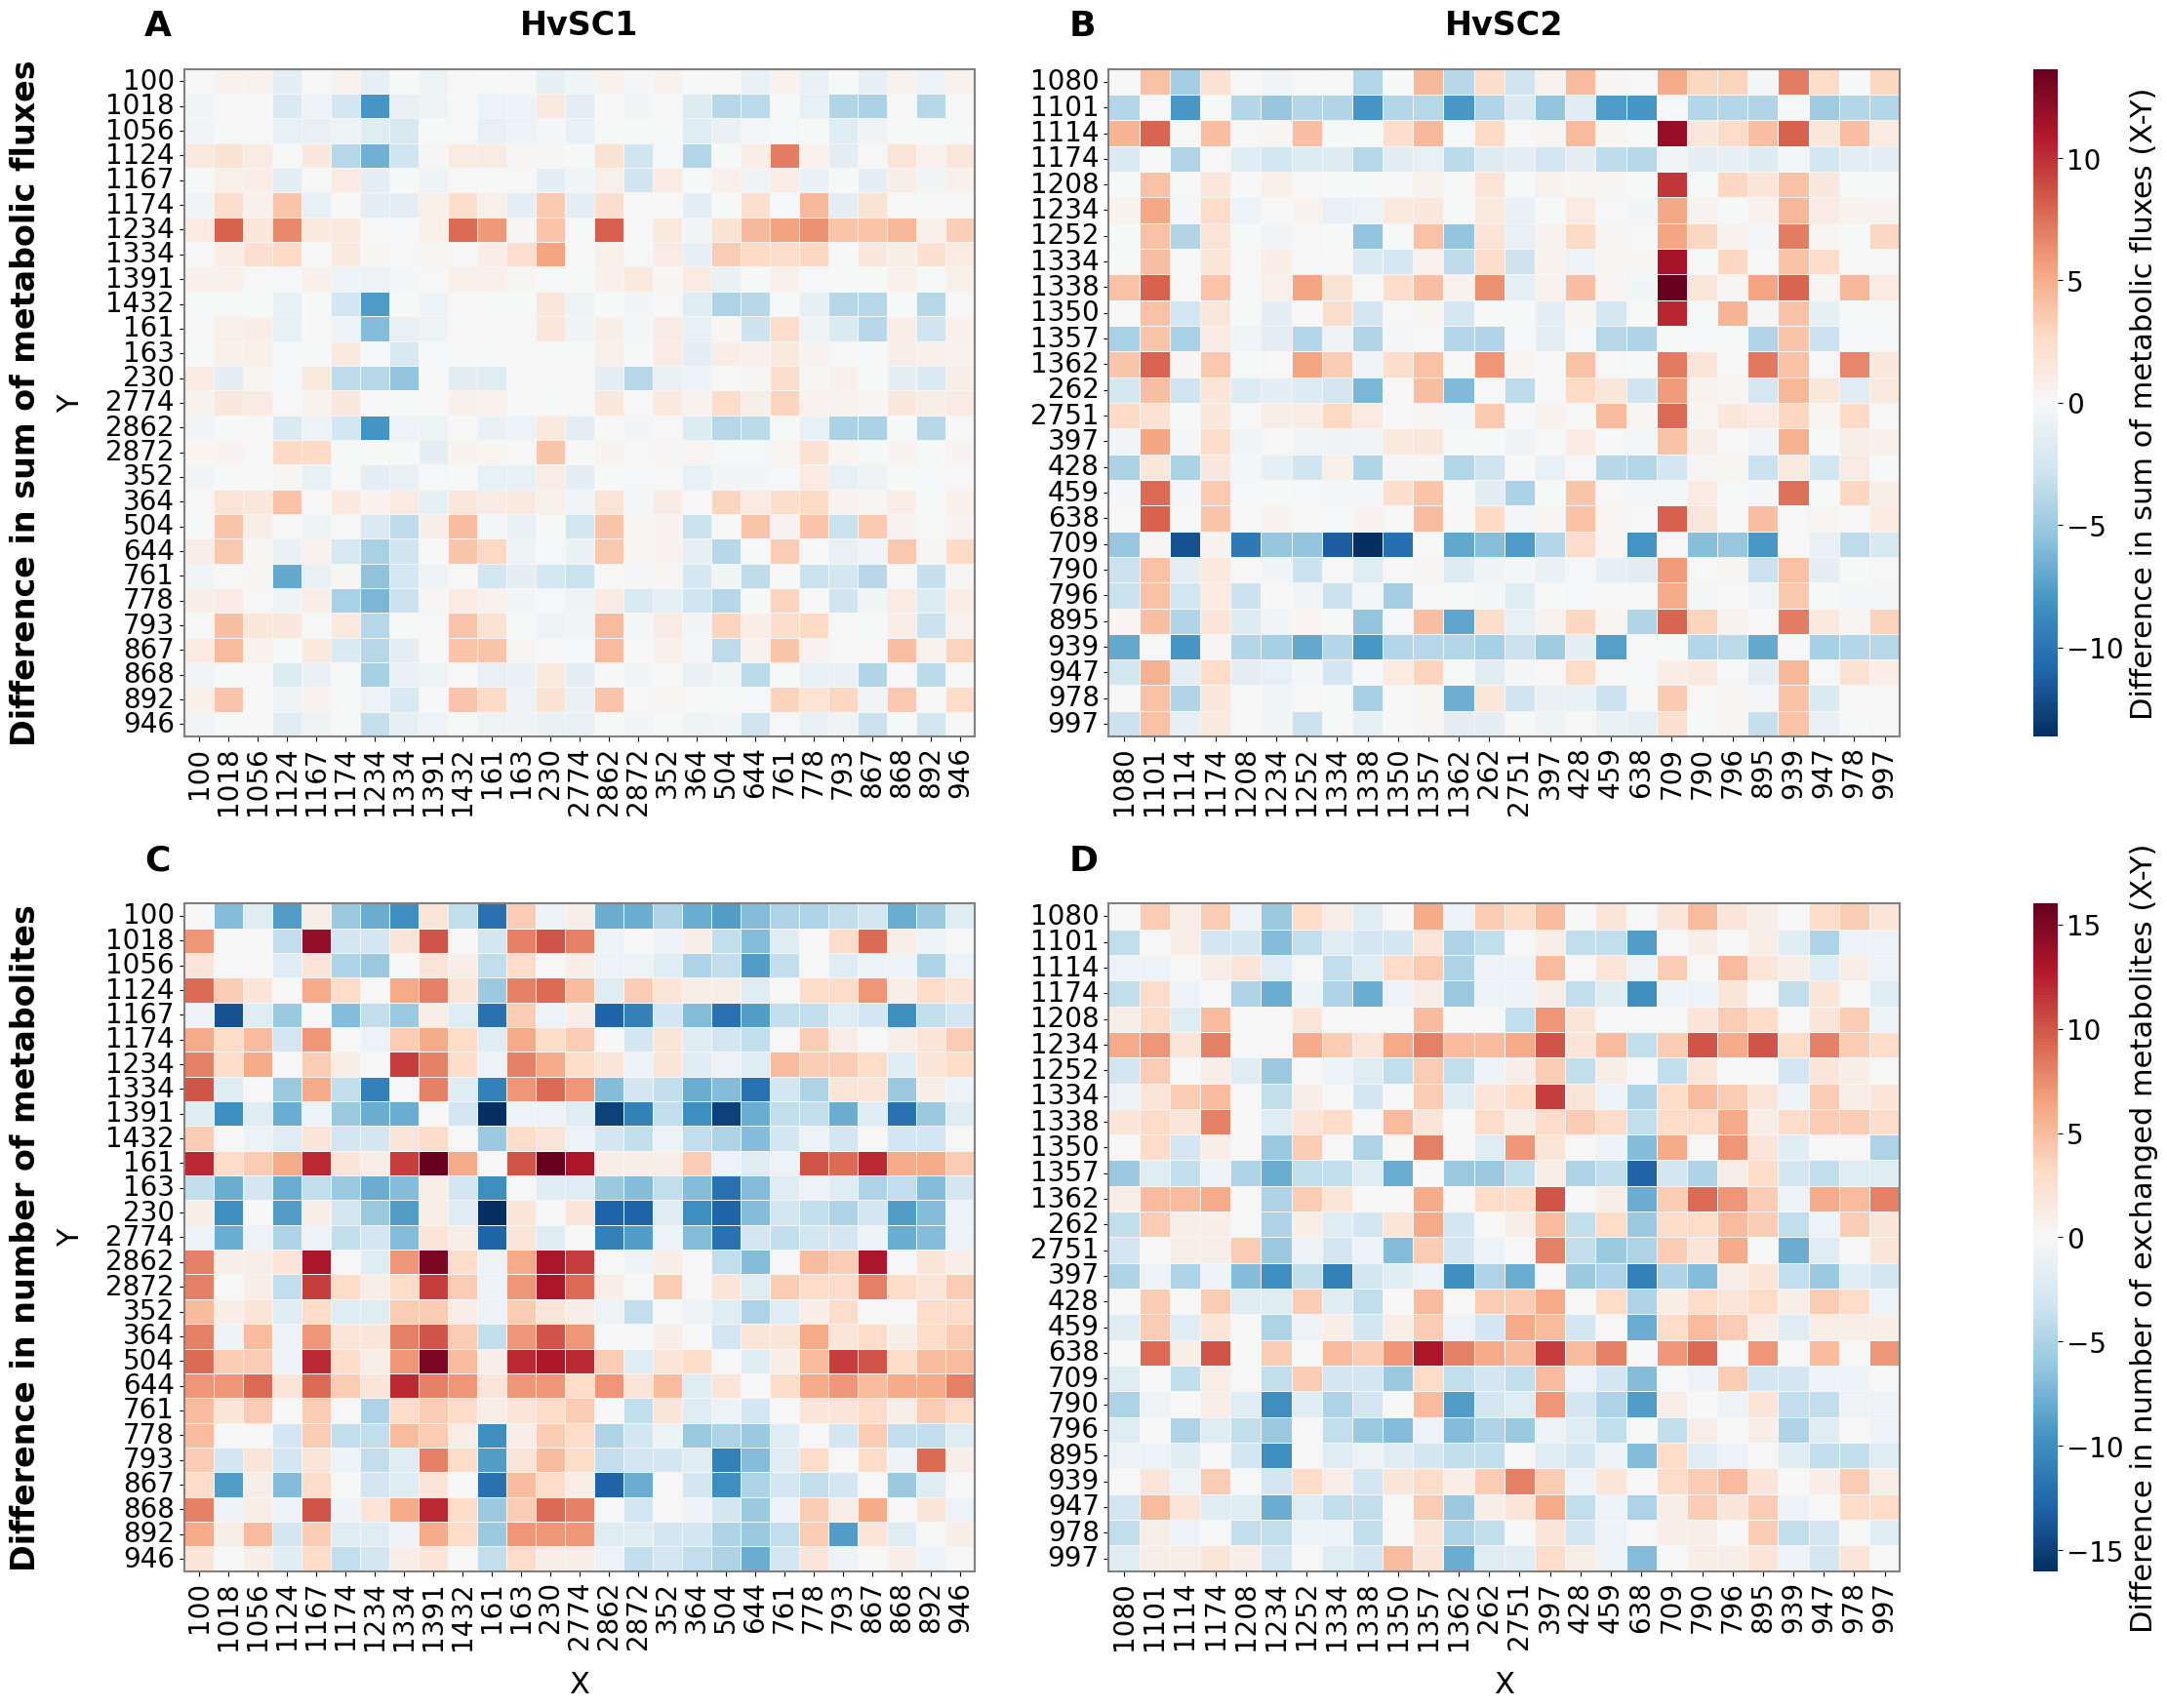
\includegraphics[width=1\linewidth]{fig/Combined_balance_nmets_flux_heatmap}
	\caption[Symmetry of pairwise metabolic interactions]{Symmetry of pairwise metabolic interactions. The heatmaps show pairwise cross-feeding interactions in scope of magnitude (A, B) and number of exchanged metabolites (C, D). HvSC1 is more asymmetric in the number of exchanged metabolites but exhibits higher symmetry in the exchanged metabolic fluxes compared to HvSC2.}
	\label{fig:balance_metabolicexchanges}
\end{figure}

\section{Drop-out experiments}
Previous analyses showed that both communities rely heavily on metabolic exchanges and indicate certain strains that might hold special importance in community structure. This raises the question how the removal of individual strains affects community behaviour. Therefore, to address my third research question, I generated drop-out communities by removing one member at a time and examined resulting changes in community and individual growth rates. 
\\


\begin{figure}[H]
  \centering
  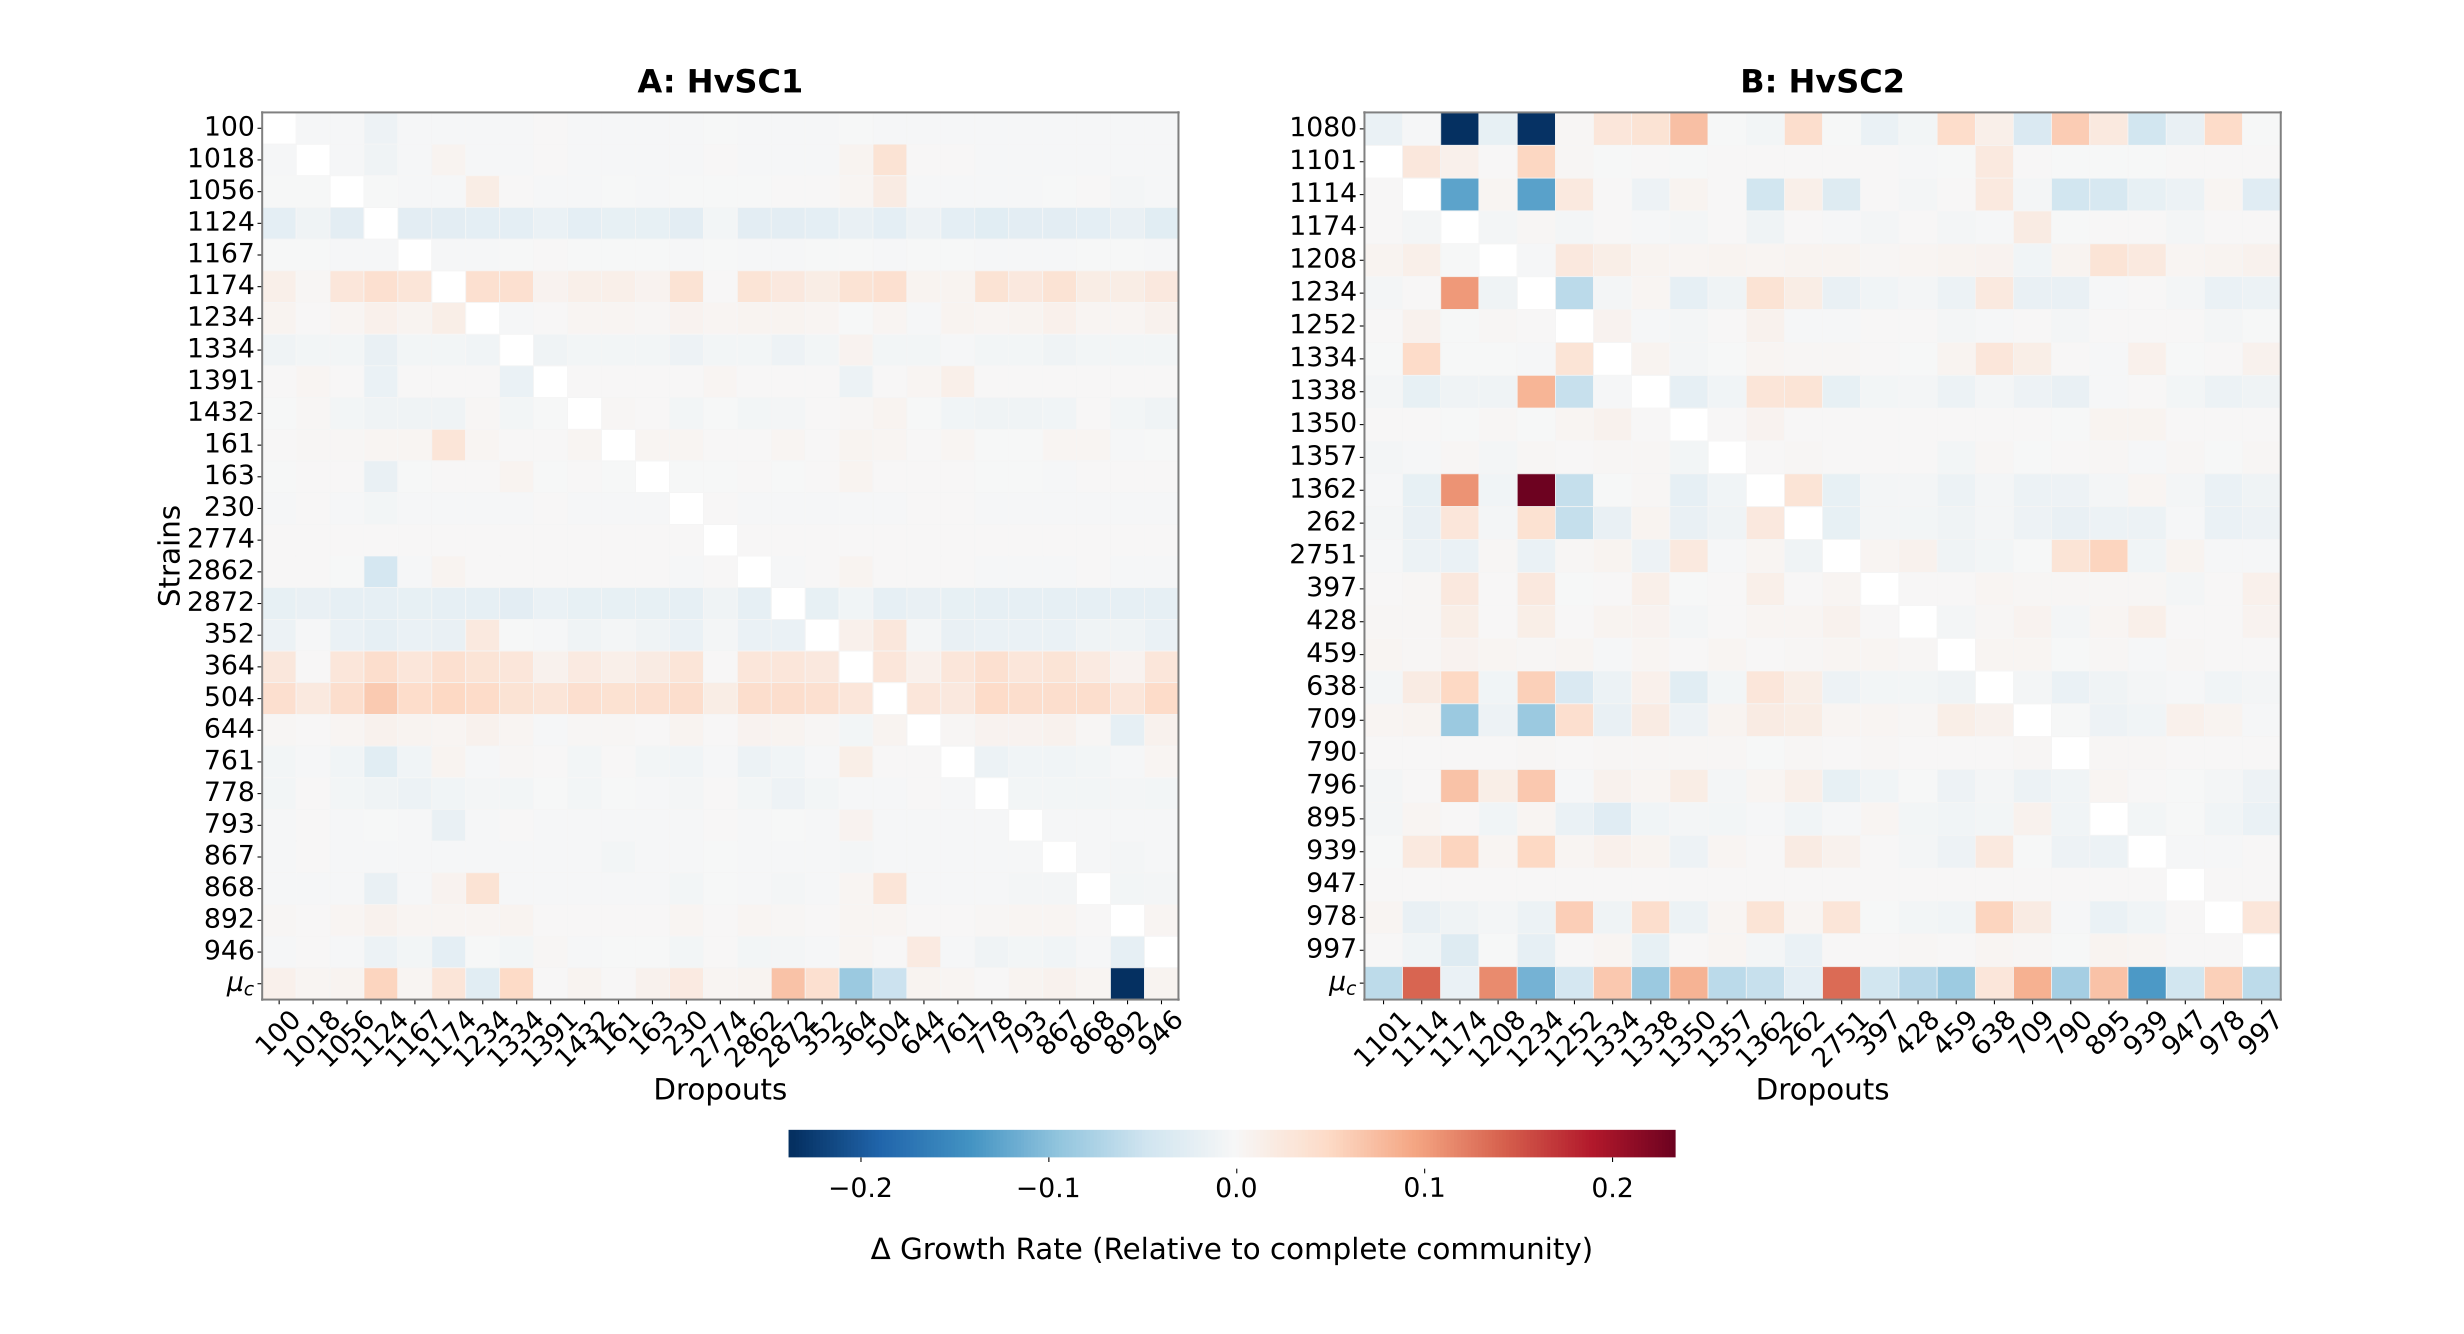
\includegraphics[width=1\textwidth]{fig/Dropout_growthrates.png}
  \caption[Impact of single-strain drop-outs on strain-level and community growth rates]{Impact of single-strain drop-outs on strain-level and community growth rates. Heatmaps for (A) HvSC1 and (B) HvSC2 display the change in growth rate ($\Delta$ Growth Rate) relative to the complete community baseline. Individually removed strains are listed on the x-axis, while remaining strains are shown on the y-axis. The bottom row ($\mu_c$) displays the net effect of each drop-out on overall community growth. Red hues indicate increased growth rates relative to the complete community, blue hues indicate reduced growth rates.}
  \label{fig:dropout_growth}
\end{figure}
The core community’s growth decreases by 5\% upon the removal of strain 892. Aside from strain 892, individual drop-outs had minimal impact on HvSC1's community growth. In contrast, the growth rate of the trait-optimised community (HvSC2) fluctuated largely depending on which species was removed (Fig. \ref{fig:dropout_growth}B, bottom row). In HvSC1, a subset of strains stands out by consistently responding to any member's removal compared to the complete community: strains 1174, 364 and 504 always grew more, whereas 1124 and 2872 grew less. No such generalised strains are detected in HvSC2 and its individual strain growth is very little affected by single-strain drop-outs. HvSC2 exhibits wider spread pairwise dependencies. In particular strains 1174 and 1234 displayed strong antagonism toward strains 1362 and 796, and cooperative interactions with strains 1080 and 1114. 
Overall, the drop-out experiments show that the core community is, under the exclusion of its keystone 892, less reliant on the presence of a single strain than the trait-optimised community, which’s growth rate fluctuates notably upon single-strain removal.

\subsection{Potential keystone strain 892}
Since I identified strain 892 as a potential keystone species in the drop-out experiments, I further analysed its metabolic interactions within HvSC1. Strain 892 engages in a total of 563 metabolic interactions within the community, which make up 5.32\% of all community interactions. It exclusively secretes two siderophores (Ferroxamine and Mycobactin T), among aromatic ring derivatives and pH regulating compounds (3-Oxoadipate and 2-Dehydro-D-gluconate). To the 26 fellow members of its community 892 provides a total of 47 metabolites, from which nitrate, aromatic nitro compounds, arginine, protoheme, and acetaldehyde are most frequently exchanged. In return, it accepts CO2 from all other community members as well as glycine betaine, cysteine, nitrite and ammonium. 
To test if 892 could stabilise the growth of the trait-optimised community, I performed a drop-in experiment, introducing 892 into HvSC2. The drop-in increased community growth rate by 8\%, to 6.437$\text{h}^{-1}$. Median individual growth rate did not change, rather the values spread more widely across the whole range, clustering less around the median and more toward the extremes ($IQR_{HvSC2} = 0.089$, $IQR_{Drop-In} = 0.172$) (Fig. \ref{fig:dropin_growth}). This indicates that the addition of 892 benefits only a subset of the community while limiting others.
\\



\begin{figure}[H]
  \centering
  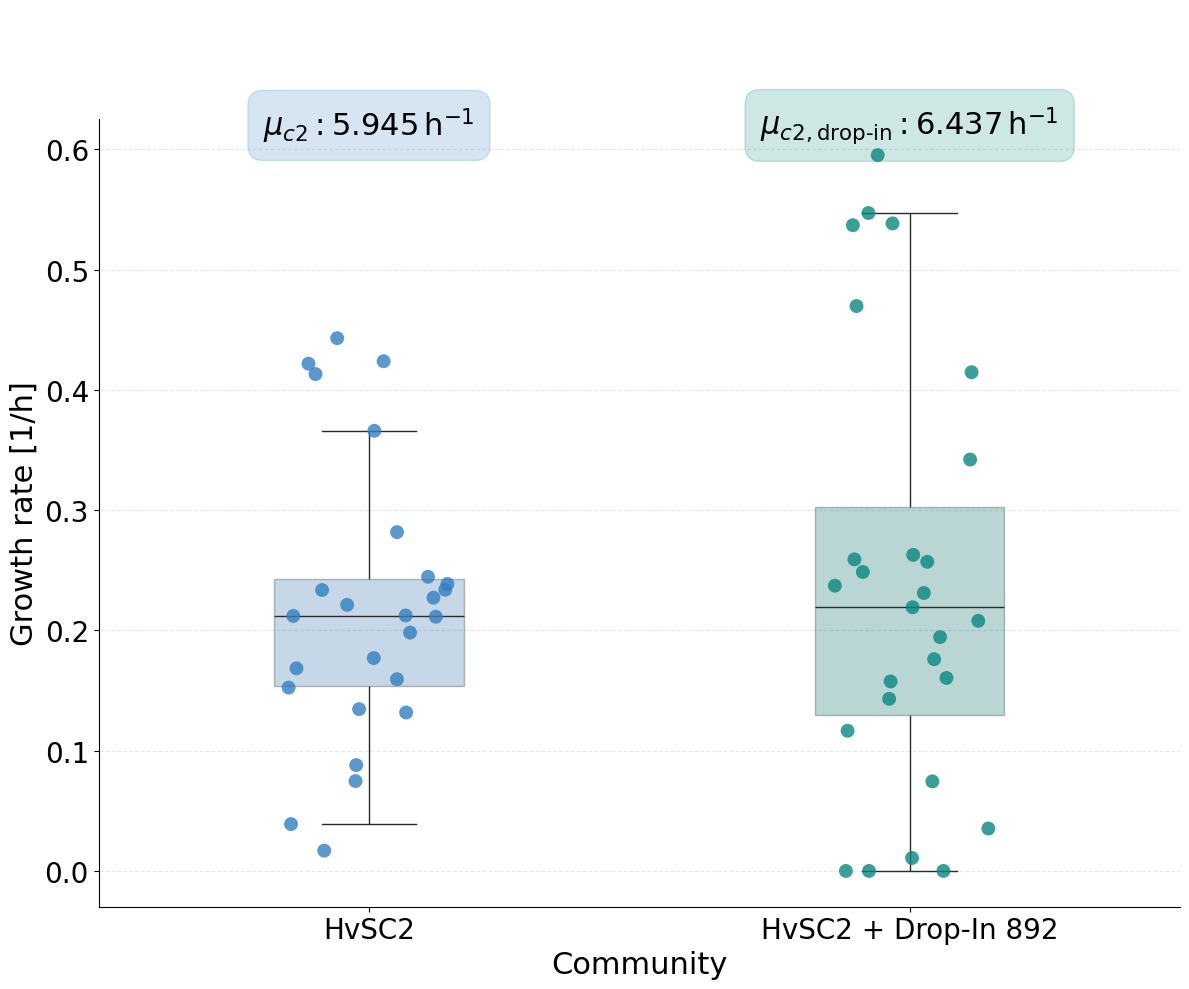
\includegraphics[width=1\textwidth]{fig/DROPIN892_Individual_growthrates_boxplot_l2pfba.png}
  \caption[Impact of drop-in strain 892 on HvSC2's growth]{Impact of drop-in strain 892 on HvSC2's growth. Comparison of individual taxon growth rates HvSC2 and HvSC2 + 892 (Drop-In 892) on completed apoplastic fluid medium. Community is indicated by colour: HvSC2 (blue) and Drop-In (dark green). HvSC2+ Drop-In 892 shows higher community growth rate $\mu_{c2, \text{drop-in}}$ compared to $\mu_2$, but growth rates are more spread, showing that the drop-in only benefits a subset of HvSC2's members.}
  \label{fig:dropin_growth}
\end{figure}

I analysed the metabolic interactions of 892 within the drop-in community, to find potential key metabolite exchanges underlying this altered growth behaviour. The metrics quantifying metabolic interactions changed only slightly (MRO: -0.003, MIP: +0.002, fMIP: +0.005).  Within the drop-in community, 892 engages in a total of 122 interactions and provides 11 metabolites, of which acetaldehyde, L-glutamate, ammonium, and nitrate are most frequently received. However, the strains receiving the highest number of metabolites or the largest total flux are not necessarily those that grow best, indicating that the observed improvement in growth cannot be attributed to metabolic exchange alone.
All in all, introducing strain 892 to the trait-optimised community increased overall community growth but made growth more imbalanced across members, an effect which can not be fully explained by 892's metabolic exchange patterns. 
% !TeX spellcheck = en_EN-EnglishUnitedKingdom
\chapter{Discussion}
This thesis aimed to understand the impact of assembly strategy on SynCom behaviour. After reconstructing and curating genome-scale metabolic models, simulating on apoplastic barley root medium showed that the models captured core metabolic functions and underlined the importance of community interactions in enabling growth, addressing the first research question. Analyses of niche overlap and cross-feeding behaviour highlighted different priorities between the communities and answering the second research question. Drop-out simulations demonstrated different robustness in growth to the removal of certain community members and revealed strain 892 (\textit{Bosea sp.} F3-2) as a potential keystone species, addressing the third research question. Together, these findings establish a basis for the answer of the fourth and fifth research questions, which require more literature context. 

\section{Metabolic interactions\textit{ in vivo} vs \textit{in silico}}

Comparing the \textit{in silico }findings to experimental results \textit{in planta}/\textit{in vitro} contextualises and potentially validates them. The two experimental frameworks investigate complementary interaction types: \cite{mahdi_low_2026}'s experiments primarily targeted antagonistic interactions, whereas GEM analysis focused on cooperative interactions. Consequently, the reconstructed communities show overall much weaker antagonistic interactions than reported \textit{in vitro}. For example, the drop-out simulations showed very few strains whose absence lead to widespread growth increases in others, underrepresenting the strongly antagonistic strains observed experimentally. Mechanisms of microbial antagonism are largely attributed to the production and secretion of antibiotics, bacteriocins, and toxins (\cite{garcia-bayona_bacterial_2018}), but the accurate representation of the producing biosynthetic pathways in GEMs remains a challenge. Databases lack information on reactions associated with secondary metabolism and these pathways are typically poorly annotated (\cite{qiu_flux_2023}). The representation of antagonistically acting metabolites in GEMs poses another challenge. Inhibiting a reaction upon the presence of a certain compound requires more complex constraints. As a result, the analysis conducted \textit{in silico }focussed on cooperative interactions which complicates the comparison to existing experimental data of the framework. Competition-based modelling approaches such as generalised Lotka-Volterra or MacArthur Consumer-Resource models could be used to complement the cooperative analyses and aid in the understanding of antagonistic interactions (\cite{van_den_berg_ecological_2022}).
\\


\textit{Hv}SC1 distributes its metabolic interactions across a broad set of smaller, more evenly-sized exchanges, while \textit{Hv}SC2 concentrates its interactions into fewer, higher-magnitude dependencies. \textit{Hv}SC1’s broad, shallow exchange strategy is, as expected, more robust to perturbation, since the loss of any single interaction means the loss of only a small fraction of a strain's total metabolite requirements, whereas a narrow, high-magnitude strategy creates more critical dependencies whose loss cannot easily be compensated by the remaining network.
One important assumption to keep in mind is that in all analyses, both \textit{in vitro }and\textit{ in silico}, all community members are equally abundant. While this framework allows constant evenness across both communities, it limits the applicability of both communities’ behaviours in practice, as natural systems are characterised by uneven and widely spread abundances (\cite{dawson_small_2017}).

\section{Keystone species}
Keystone species are defined as highly connected taxa, which play a unique and central role in community structure and function (\cite{banerjee_keystone_2018}). Because their influence is disproportionate to their abundance, removing them can cause profound systemic shifts (\cite{carlstrom_synthetic_2019}). Based on this framework, strain 892 can be termed a keystone species: It is a central exchange partner to its community members, its removal strongly decreases community growth, and its addition increases community growth. This pattern mirrors reports in other SynComs where a single strain's removal disproportionately destabilises the network (\cite{krumbach_metabolic_2021, sun_metabolic_2023}).
\\


Strain 892 has been identified as \textit{Bosea sp.} F3-2, and is a member of the \textit{Boseaceae} family. First isolated from the tobacco rhizosphere, this strain has been presented as a promising biocontrol candidate against quorum-sensing pathogens (\cite{zhang_aidb_2019}). Members of the genus \textit{Bosea} are classified as chemolithoheterotrophic, which is reflected in strain 892's metabolic profile. As a chemolithotroph, it is able to obtain energy from inorganic compounds, which has been proven for thiosulfate but has not been previously documented for the GEM-predicted nitrogen compounds (\cite{das_oxidation_1996}). Most notable is its involvement in heterotrophic nitrification, the oxidation of ammonium via nitrite to nitrate. This is consistent with literature emphasising how the substrate availability in the rhizosphere enables this pathway (\cite{martikainen_heterotrophic_2022}), through which strain 892 acts as a detoxifier by removing toxic nitrite and provides a nitrogen source to its fellow community members. 
The role as a central exchange partner is further supported by Strain 892's exclusive secretion of two siderophores. These compounds function as costly public goods that are frequently shared and also shape growth behaviour by mediating iron acquisition across the wider community (\cite{kramer_bacterial_2020}). 
\\


Strain 892’s beneficial role in a community is underscored by the increase in community growth upon the addition of strain 892 to the trait-optimised community. It facilitates growth for a subset of strains, for example by providing nitrate, while others grow less. The increased spread of individual growth rates upon 892's drop-in is notable because it runs counter to the compressive tendency of the L2-norm regularisation discussed below, which pushes growth rates toward equality rather than apart. This suggests that the spread in growth rates reflects a true biological effect of 892's addition. The change in growth behaviour is not purely caused by 892’s influence on metabolic exchanges, as the most frequent receivers are not necessarily the strains with the most improved growth. This implies that 892 reshapes community dynamics via more complex mechanisms than can easily be explained by its direct participation in pairwise cross-feeding analyses.
\\


In the \textit{in vivo }analysis, strain 892 is a persistent member of the core community over a six-day time period, and shows inhibition of only one strain in inhibition assays (\cite{mahdi_low_2026}). As the authors did not investigate detailed mechanisms of microbial cooperation or conduct community-wide drop-out experiments, strain 892 did not stand out. In the computational analysis, strain 892 is really only highlighted as a potential keystone upon its removal.  Besides the fact that strain 892 exchanges metabolites with all \textit{Hv}SC1 community members, it does not stand out as a structural outlier within its community when comparing its exchanges in number of metabolites, flux magnitude or symmetry. A validation of its keystone role in \textit{in vitro}/\textit{in planta} drop-out and drop-in experiments, followed by the analysis of changes in community behaviour and function would underline this predicted result.  
While it is clear that 892 has a special role within the communities, the exact underlying working mechanisms remain unclear. Results obtained from GEMs can be used to guide further experiments, as they highlight potential interesting behaviours which can be looked into experimentally. This will improve our understanding of keystone species, which remains a central task in plant-microbe modelling, as such keystone strains can be used to enhance host performance and community diversity (\cite{krumbach_metabolic_2021}).

\section{Community stability}
Efficient, innovative and sustainable applications of SynComs in agriculture require stable communities. It is therefore crucial to understand the drivers of stability and also how stability can be achieved in comparatively unstable communities. There are various ways to define stability in ecology. As assessing time-resolved processes with the used GEMs is hard, this thesis investigates stability indicators, namely balanced communities’ exchanges, and a community’s response to exclusions/additions. These further potentially drive stability, aiding stable composition over time, and help to improve the mechanistic understanding of long-term robustness. Literature highlights metabolic exchanges as a key driver of stable microbial communities (\cite{zelezniak_metabolic_2015}), consequently factors enhancing cooperation can also improve stability (\cite{wang_narrow-spectrum_2025}). Symmetry in both competitive and cooperative interactions promotes stability (\cite{butler_stability_2018}). Furthermore, it has been shown that communities with keystone taxa maintained more stable compositions and species abundances (\cite{liu_keystone_2025}). Based on this framework, the stability indicators of the two SynComs can be compared. 
\\


Both communities heavily rely on cross-feeding, however, the structure of the exchange networks differ. \textit{Hv}SC1 exchanges more metabolites per strain pair, showing greater average connectedness and lower, more symmetric exchange fluxes, while \textit{Hv}SC2's exchanges are comparatively less diverse and heavily asymmetric. Following \cite{butler_stability_2018}, this symmetry indicates greater stability for \textit{Hv}SC1, a prediction supported by the drop-out experiments, where only 892's removal noticeably perturbed \textit{Hv}SC1, while \textit{Hv}SC2's growth fluctuated more across all drop-outs. This implies that greater connectivity as well as symmetric and widely distributed interactions buffer metabolic needs and allow for adjustments to new conditions such as the removal of community members. Linking this back to functional redundancy, this shows that not all community members are strictly required for community stability, if a strain’s function is redundant with remaining members (\cite{allison_resistance_2008}).
\\


In both SynComs all members are equally abundant, hence species evenness, which can be one factor in establishing stability (\cite{wittebolle_initial_2009}), is also held constant across both communities. Consequently, evenness cannot account for the observed difference in robustness. The differences of \textit{Hv}SC1 and \textit{Hv}SC2 must therefore stem from the communities' other structural properties, such as connectivity or exchange flux symmetry. 
Keystone strains have been shown experimentally to support stability by (at least) two mechanisms: structural centrality, where highly connected keystone taxa provide redundant pathways that buffer the network against member loss (\cite{liu_keystone_2025}), and specialised function, where a keystone performs a metabolic role, that can not be substituted by other community members (\cite{iram_deciphering_2025, xun_specialized_2021}). Strain 892’s metabolic interactions exert influence on stability mainly through the latter: its role in nitrogen cycling, which exemplarily stands out upon its removal, demonstrated that its functional contribution can not be substituted by any other strain. 
\\


The investigated perspective on stability differs between the computational and experimental framework: While \cite{mahdi_low_2026} focused on stability over time, my analyses provide deeper understanding of stability indicators that may also aid establishing stability in the first place. Combining both approaches shows that the predicted stabilities of the \textit{in silico} communities align with the \textit{in planta} experimental results (\cite{mahdi_low_2026}). \textit{In planta}, \textit{Hv}SC1 largely retained its initial composition over a longer time, showed a larger number as well as more cooperative interactions and exerted higher environmental robustness. This is mirrored in the reconstructed \textit{Hv}SC1’s behaviour: the community is more balanced in its exchange fluxes as well as less impacted by single strain drop-outs, a result further supported by literature showing that an established community is more difficult to perturb (\cite{carlstrom_synthetic_2019}). In contrast, \textit{Hv}SC2 showed higher antagonism and major changes in community composition over time\textit{ in planta}, which is again consistent with the reconstructed \textit{Hv}SC2’s asymmetric exchanges and decreased robustness in drop-out experiments. All together, the results underline that symmetric metabolic interactions and the presence of stabilising keystone taxa are indicators of stable communities.

\section{Co-occurrence vs. trait-based: Impact of assembly strategies on community behaviour}\label{sec:assembly_strat_discussion}
The two SynComs clearly show how assembly strategy impacts community behaviour. The core community, which was assembled based on co-occurrence, demonstrates that co-occurrence promotes balanced community behaviour and robustness to changing conditions. Further, its more balanced individual growth rates are consistent with expectations from co-existence theory: selection acts against large asymmetries which would exclude slower-growing members long-term, to ensure stability over time (\cite{chesson_mechanisms_2000}). In \textit{Hv}SC1 these selection processes may already have taken place, whereas the trait-optimised community has not undergone this development, explaining why \textit{Hv}SC2 shows a more unevenly distributed exchange network with larger asymmetries in its individual growth rates. This distinction links nicely to a broader pattern in the literature: communities assembled for functional complementarity alone, without regard for ecological compatibility, tend to be less stable than those built around natural co-occurrence (\cite{de_souza_microbiome_2020}).
\\


The impact of assembly strategy goes beyond stability. Essential to a community’s effectiveness in promoting plant productivity and protection is its colonisation strength, efficient metabolite usage and balanced cooperations within the community. Literature shows that native core microbiomes often outperform other communities in exactly these aspects, resulting in greater potential to promote plant growth and yield (\cite{de_souza_microbiome_2020, zhou_superiority_2024}). 
\\


These results suggest a practical design approach: basing the design of trait-prioritised SynComs on native core communities that are commonly found across soils helps to overcome limitations in establishing stable host-microbiome relationships and scalability caused by narrow host and environment adaptability, i.e., a community only being stable in one specific environment (\cite{zhou_superiority_2024}). Further this would enhance the colonisation activity of SynComs, as outcompetition with naturally occurring bacteria can be prevented (\cite{de_souza_microbiome_2020}). The selected traits for \textit{Hv}SC2 by \cite{mahdi_low_2026} focused on plant-growth promoting or pathogen-protecting traits. In the future, the performance and stability of community-host associations could be improved by screening for strains that are enriched in genes that aid colonisation, such as those involved in boosted carbon metabolism (\cite{de_souza_genome_2019}). Ultimately these approaches point towards a hybrid assembly strategy, which combines core and trait-optimised communities, to help to realise the full potential of SynComs in agriculture. 

\section{Assumptions in model reconstruction and simulation}

\subsection{Model reconstruction quality and remaining curation challenges}
As shown by the MEMOTE scores, the curation process clearly improved the quality of the models and thus their accuracy in the representation of biological reality. Missing annotations cause the main gap to a “perfect score”. Although these gaps affect model quality metrics, annotations are less critical to functional predictions than network consistency and connectedness. 
\\


Comparing predicted to experimentally determined growth rates informs about plausibility of the models’ growth behaviour. In a community modelling context, this comparison is hard, as the community growth rate is not one experimentally measurable quantity but calculated based on different underlying metrics. The calculation approach, for example summing abundance scaled growth rates, substantially affects the community growth rate. Further, individual growth rates within the community context are difficult to compare to monoculture measurements in laboratory conditions, since a community model has access to a much larger combined resource pool than any single organism would in isolation. For reference, the fastest growing reported bacterium grows at a rate of $2.81 \,\text{h}^{-1}$ in optimal laboratory conditions (\cite{lee_functional_2019, lieven_memote_2020}), rhizospheric bacteria are reported with growth rates around $0.2-0.3 \,\text{h}^{-1}$ (\cite{lopez_growth_2023}). The abundance-scaled predicted growth rates fall within this range, but the unscaled ("raw") growth rates exceed biologically plausible values. Unrealistically high growth rates are one of many artifacts arising from uncertainties in various steps in GEM reconstruction and analysis. Uncertainties in genome annotation arise, as the mapping of homologs may be uncertain, or the reconstruction and interpretation of GPRs erroneous. This necessitates gap-filling, which is inherently uncertain because the reactions added are generally not supported by genomic evidence. One example, directly influencing growth rates, are sparsely characterised transport reactions, which lead to many pseudo-reactions with incomplete substrate specificity (\cite{bernstein_addressing_2021}). This causes thermodynamically impossible energy-generating cycles (EGCs), which allow for the production of energy metabolites (e.g., ATP or NADPH) without nutrient consumption, thereby inflating growth of a model. This partly explains the increased raw individual growth rates. One approach to resolve EGCs involves a variant of the GlobalFit algorithm, which suggests a minimal number of reaction removals that eliminate all EGCs. The algorithm is very computationally expensive and hence only applicable to small models (\cite{fritzemeier_erroneous_2017}). Even though this algorithm is almost 10 years old, there are no viable fully automated alternatives for large-scale GEMs, leaving the resolution of EGCs a matter of manual curation.
\\


Formulating the biomass objective function is another source of uncertainty. Very few experiments quantify the exact composition of a bacterium's biomass. Like many other tools, CarveMe uses a model organism’s biomass composition as a template, despite the importance of organism- or even strain-specific composition of the biomass (\cite{xavier_integration_2017}). Failure of menaquinol synthesis in strain 895 shows the problems with this generalised template approach. Although I only corrected the biomass function for this one strain, as all others functioned as expected, a thorough re-evaluation of all other biomass objective functions would ensure true biological replicability. Determining the exact biomass composition calls for large amounts of metabolomics data. Generating these datasets requires high-throughput workflows, such as automated, AI-guided robotic laboratory platforms (Jensen et al., 2025). The resulting experimental data can then be integrated into software tools like BOFdat (\cite{lachance_bofdat_2019}), which algorithmically infer accurate biomass stoichiometry directly from multi-omics data.
\subsection{Medium and its influence}
The composition of the growth medium has a major influence on bacterial growth rates \textit{in vitro} and impacts the behaviour of the communities \textit{in silico}. Consequently, defining a physiologically plausible and well-characterised medium is a crucial prerequisite for constraining community simulations. The medium used in this thesis is based on metabolomics data collected seven days post inoculation from the barley root apoplast by \cite{saake_ergosterol-induced_2025}. The authors also provided data from eight days post inoculation, which shows a substantial metabolic shift compared to the data obtained seven days post inoculation. These fast metabolic changes highlight the need for higher-resolution time-series datasets, and suggest averaging strategies across broader experimental replicates to construct robust baseline media definitions. Furthermore, spatial differences in metabolite abundance along the root may be another influence on experimental data (\cite{loo_sugar_2024}). Another challenge arises in the mapping of \textit{in planta }detected metabolites to their counterparts in the GEMs, as not all metabolites are listed in the BiGG database. Consequently, as the model reconstruction is based on BiGG, these metabolites can not be represented within the models. Additionally, not every metabolite found in the medium is present in the model, which requires gap-filling as well as including detailed knowledge about correctly absent pathways. During my medium generation process I identified 15 metabolites detected \textit{in planta}, which were not found in the GEMs. Moreover, defining realistic component uptake bounds remains challenging, as not much quantitative kinetic and transport data is available. These limitations highlight the need for more comprehensive metabolomic profiling and demonstrate that all results must be evaluated in the context of their environment.

\section{Limitations and relevance of the optimisation method} 
The results obtained in this thesis must be carefully interpreted, especially under the background of the employed constraint-based approach, underlying model quality and preceding assumptions. Contrasting to experiments \textit{in vivo}, the simulations do not include replicates. Even though the solution space is large, every optimisation returns a single maximal growth rate for every model, which might not capture natural variability. Consequently, standard statistical evaluation and significance testing, as typically applied to experimental datasets, were not performed here. Approaches such as flux variability analysis and alternative optima testing allow for statistical comparisons and present an aspect future work could investigate but were beyond the scope of this thesis.

\subsection{Limitations of (p)FBA}
The FBA method has its own limitations. Central to biologically relevant results is the choice of the objective function of a model. While for the exponentially growing community scenarios evaluated in this thesis, biomass maximisation remains a physiologically relevant proxy, depending on the research question this might change and is not achievable or preferable in every environmental condition (\cite{raman_flux_2009, schuetz_systematic_2007}). Furthermore, classical FBA operates under steady-state assumptions without integrating metabolic kinetics or enzyme allocation constraints. Consequently, the framework cannot account for proteomic capacity limitations, which can lead to unrealistic flux predictions. One example are non-growing or dormant strains carrying unphysiologically high metabolic fluxes. Merging FBA with kinetic methods in a dynamic FBA (dFBA) and non-linear optimisation approaches can help to overcome these limitations by predicting dynamic model behaviour (\cite{de_oliveira_nonlinear_2023, mahadevan_dynamic_2002}).
\subsubsection{Cooperative trade-off function - relevance of optimisation method}
The behaviour of the community is strongly influenced by the optimisation strategy employed in MICOM (\cite{diener_micom_2020}). Different growth rates were observed for different optimisation strategies (Fig. \ref{fig:hvsc1individualgrowthmethods}, \ref{fig:hvsc2individualgrowthmethods}), with profound implications for the entire system. A notable example is the blocking of sugar exchanges. The detected irregular rates observed under MICOM’s \texttt{cooperative\_tradeoff()} can be traced to its numerical crossover procedure, which is triggered when the optimisation solver fails to reach optimal convergence (see Section \ref{sec:Construction and simulation of community models}). The crossover heuristic attempts to recover a sparse flux distribution, but numerical inaccuracies during this step can artificially inflate flux throughput. When the crossover function was explicitly bypassed, no discrepancies in the results were detected. 
Aside from the computational aspects, the optimisation strategy should also reflect biological reality. When predicting metabolism \textit{in silico}, the flux distribution is closest to proteomics and transcriptomics measurements, when a GEM is optimised for a minimal sum of fluxes (pFBA) (\cite{lewis_omic_2010}), which serves as a first proxy for the assumption, that an organism will only invest minimal enzyme amounts. Further, growth rates simulated under L2 regularisation correlate more with experimentally observed replication rates compared to non-regularised results (\cite{diener_micom_2020}). 
\newpage

Therefore, I defined my own optimisation function, which similarly to MICOM’s original \linebreak \texttt{cooperative\_tradeoff()} function minimises the difference between individual growth rates (L2 norm) and also the sum of fluxes (pFBA) under a certain trade-off of maximal community growth. In contrast to MICOM’s function, it bypasses the crossover strategy and accepts non-optimal, yet numeric results. Numerical results in this case are acceptable, because small numerical deviations in individual growth rates do not meaningfully alter the overall community growth being compared. 
\\


The employed optimisation strategy reduces the number of non-growing strains compared to a regular pFBA, however it does not solve the problem of non/very little growing strains still carrying fluxes. While this is not a problem for the regular \textit{Hv}SC1 and \textit{Hv}SC2 communities, it certainly influences community behaviour of the drop-in \textit{Hv}SC2 + 892, as here three strains are growing less than $\mu_i = 0.001 \,\text{h}^{-1}$. As for the drop-in community, no detailed analysis of the exchange fluxes was performed, this was not specifically corrected for. One approach to address this in the future would be to shrink a strain’s upper and lower bounds once its growth falls below a defined threshold.
\\


A critical step in all these trade-off methods is the choice of the most suited trade-off parameter $\alpha$, which controls whether the optimisation prioritises community or individual growth. In my simulations, this parameter is always one, therefore optimising for maximal community growth. Decreasing the trade-off parameter yields overall smaller and more similar growth rates for the community members (Fig. \ref{fig:hvsc1individualgrowthtradeoff}, \ref{fig:hvsc2individualgrowthtradeoff}). As the goal was to compare individual growth rates in a community context, it is essential to choose a trade-off value that enables this comparison.  
\\


Even when using the custom function, certain observed patterns can still be artefacts of the trade-off strategy. Under the L2 norm, strains with very high growth rates are pushed down, while strains with very low growth rates are pushed up. Because this compression effect is distributed across all community members, its magnitude depends on community size: removing a member redistributes the compression across fewer remaining strains, weakening the push-down effect on strong growers and similarly the push-up effect on weak growers. Therefore, the strongest and weakest growing strains in a community should show a consistent directional shift upon any member's removal, as a mathematical consequence of the regularisation, independent of any true metabolic release or competition. This closely matches the pattern observed for the five strains in \textit{Hv}SC1 that responded consistently across all drop-out experiments. To further distinguish genuine biological truths from methodological artifacts, one should compare the results of different community modelling tools such as PyCoMo (\cite{predl_pycomo_2024}) or ReMIND (\cite{oftadeh_constraint-based_2024}). 

\section{Future perspectives}
This thesis helps to understand the impact of assembly strategies on community behaviour. Analysing differences in metabolic requirements, community interactions and perturbation robustness provides a detailed characterisation of the two investigated barley SynComs and aids future SynCom design. Nevertheless, there are plenty more open questions and tasks.
\\

 
One aspect is the improvement of model quality. Even with the high quality of the presented models, further refinement is required to reduce remaining errors and inaccuracies. Accuracy would be improved by removing EGCs, customising biomass functions, as well as including more experimental data on the individual strains, their environment and their interactions would further improve model and prediction accuracy. The inclusion of temporal processes, such as the previously mentioned dFBA would not only improve individual model quality, but also enable the long-term assessment of coexistence stability.
\\

 
Generally, the results of this thesis require experimental validation because GEM-based predictions rely on simplified assumptions that may not represent microbial behaviour in a real, dynamic environment. Especially drop-out and drop-in experiments of the keystone strain 892 would tell, if the predictions made here are also applicable \textit{in planta}, which would further help to understand the role of 892 in pathogen protection. Furthermore, experiments quantifying the cooperation between community members i.e, via systematic pairwise co-culture assays, would present valuable validation of the GEMs’ predictions.
\\


To understand how these SynComs protect the plant from pathogen invasion and promote growth, simulating the whole system, including GEMs of fungal pathogens and the barley plant would be necessary. While this comes with its own challenges, such as ensuring compatible metabolite exchanges, integrating host and pathogen models with existing bacterial community models would provide important insights into plant protection and microbiota function. The obtained predictions could easily be validated using the established experimental system of \cite{mahdi_low_2026}. 
\\


Finally, the insights gained in this thesis are relevant for the efficient and successful design of SynComs. As described in Section \ref{sec:assembly_strat_discussion}, combining core with trait-selected strains improves community stability and overall function. Understanding how core- and trait-based communities behave in isolation, as investigated in this thesis, is a foundational step towards understanding how such combined approaches would work in practice. Further modelling efforts and machine learning can support SynCom assembly by aiding the analysis of high-dimensional microbial datasets, predicting microbiome stability, compatibility, and emergent functions of new combinations and supporting the identification of strains possessing target functions from large datasets (\cite{garces-ruiz_machine_2026}).


\chapter{Conclusion}

This thesis used genome-scale metabolic modelling to characterise two barley rhizospheric SynComs assembled under different strategies. These communities were a core community (\textit{Hv}SC1), assembled from co-occurring strains, and a trait-optimised community (\textit{Hv}SC2), composed of strains previously shown to promote plant growth or protection. The aim was to understand how assembly strategy shapes community structure, metabolic exchange, and stability.
Both communities relied heavily on cross-feeding to meet their metabolic requirements, but differed markedly in the structure of this exchange: \textit{Hv}SC1 showed more symmetric, evenly distributed metabolite exchanges, while \textit{Hv}SC2's exchanges were sparser and more asymmetric in flux magnitudes. Consistent with this structural difference, \textit{Hv}SC1 was substantially more robust to single-strain removal than \textit{Hv}SC2, whose growth fluctuated depending on member removal. Drop-out experiments further identified strain 892 (\textit{Bosea sp.} F3-2) as a keystone strain within \textit{Hv}SC1. These results demonstrate pronounced effects of assembly strategy on community behaviour and are in line with expectations based on experimental data and literature. 
\\


As shown here, even with remaining uncertainties e.g. in model reconstruction, constraint-based modelling can identify distinct metabolic behaviour and interaction patterns in plant-associated bacteria. The thesis also discusses limitations and opportunities to overcome these from both the computational and the biological perspective. All in all, this thesis contributes to an improved mechanistic understanding of the influence of assembly strategy on SynCom behaviour and can support the development of stable, plant-beneficial microbial communities for barley and beyond.


\printbibliography
\cleardoublepage
% !TeX root = master.tex
% !TeX spellcheck = en_EN-EnglishUnitedKingdom

\appendix
\chapter{Appendix}
\label{sec:appendix}
\raggedbottom
\section{Supplementary Figures}
\subsection{Pairwise co-consumption}
\begin{figure}[H]
	\centering
	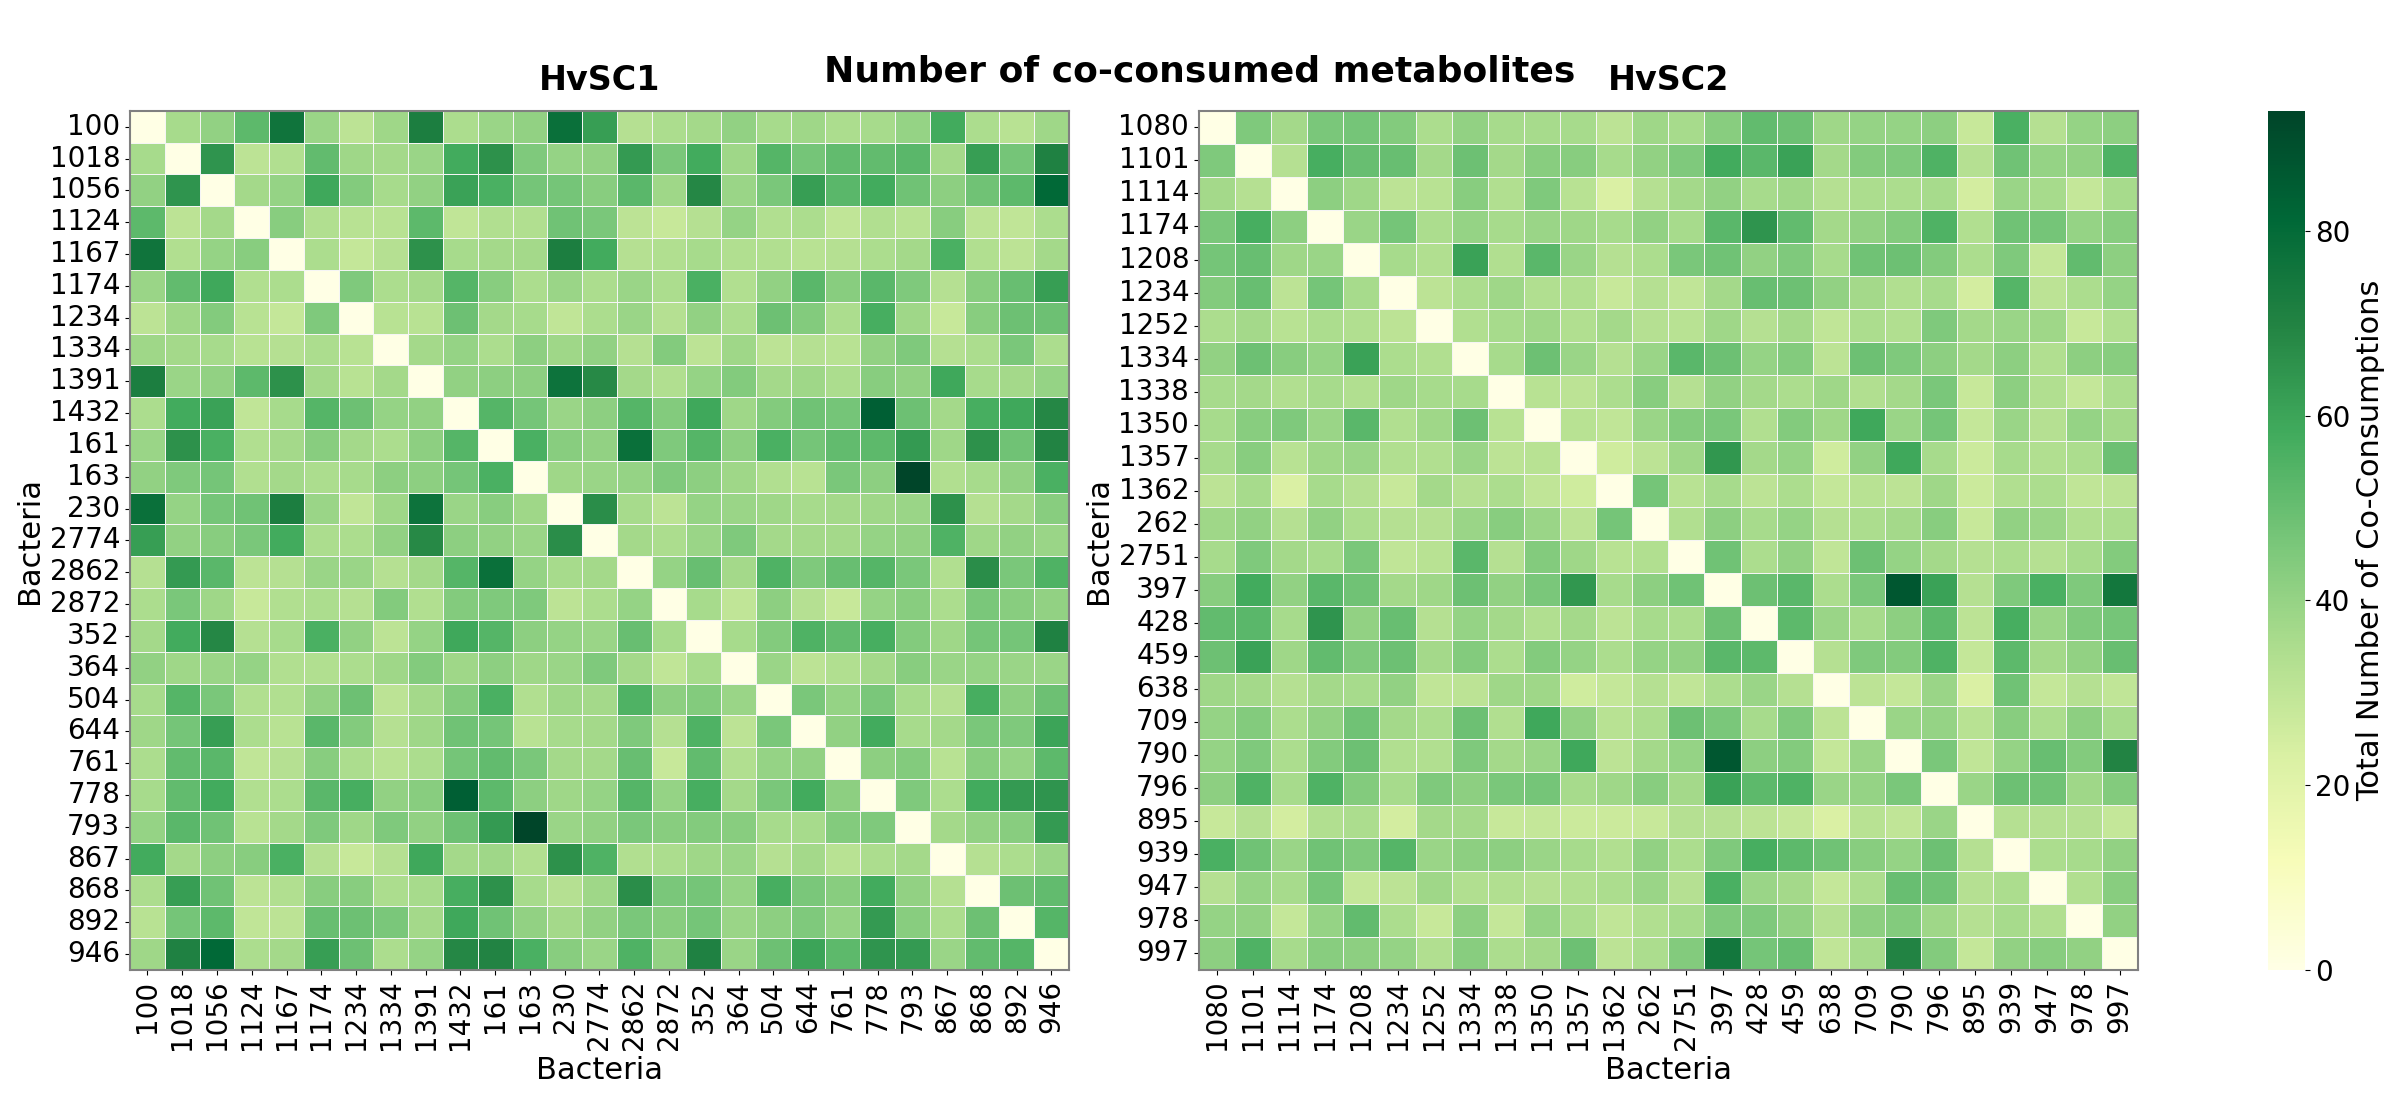
\includegraphics[width=1\linewidth]{fig/Combined_Numbercoconsumptions_heatmap}
	\caption[Number of pairwise co-consumptions]{Number of pairwise co-consumptions. Heatmaps show the total number of co-consumed metabolites for each pair of bacteria in HvSC1 (left) and HvSC2 (right). Rows and columns represent bacterial taxa, and darker green indicates a greater number of co-consumed metabolites. HvSC1 shows more co-consumed metabolites, compared to HvSC2.}
	\label{fig:combinednumbercoconsumptionsheatmap}
\end{figure}

\subsection{Medium generation process}

\begin{figure}[H]
	\centering
	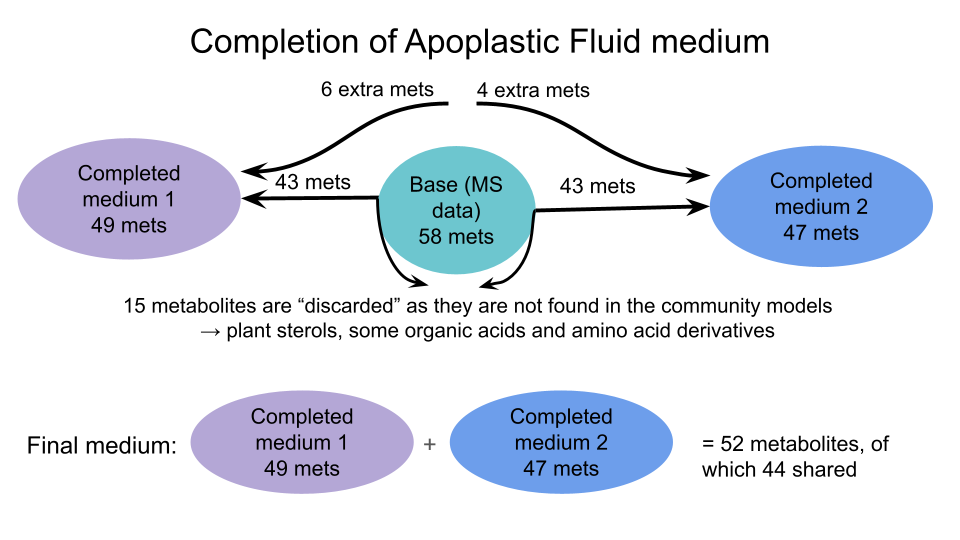
\includegraphics[width=1\linewidth]{fig/medium_completion_process}
	\caption[Medium completion process]{Completion of the apoplastic fluid medium. The base medium contained 58 metabolites derived from the MS data. After excluding 15 metabolites that were not detected in the community models, 43 metabolites were retained for each completed medium, with 6 additional metabolites added to medium 1 and 4 additional metabolites added to medium 2. The resulting media contained 49 and 47 metabolites, respectively. Combining both completed media yielded a final medium containing 52 unique metabolites, of which 44 were shared between the two communities.}
	\label{fig:medium_completion}
\end{figure}

\subsection{Impact of optimisation strategy on individual growth rates}

\begin{figure}[H]
	\centering
	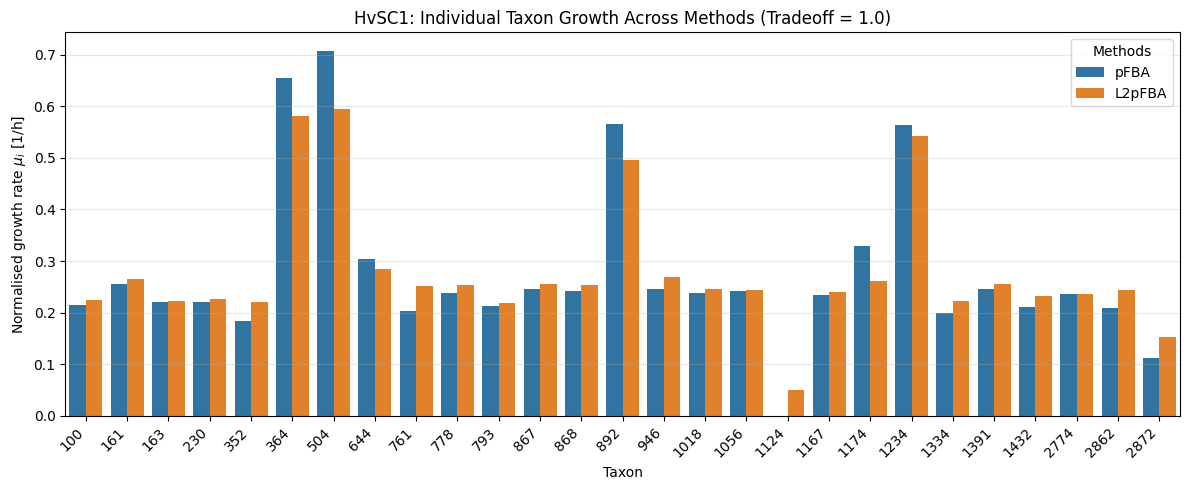
\includegraphics[width=1\linewidth]{fig/HvSC1_individual_growth_methods}
	\caption[Impact of optimisation strategy on individual growth rates of HvSC1]{Impact of optimisation strategy on individual growth rates of HvSC1. Barplot showing scaled $\mu_i$ of HvSC1 at trade-off $\alpha = 1.0$ for different optimisation strategies: pFBA only (blue) and L2-regularisation + pFBA (orange). L2-regularisation yields less extreme growth rates and ensures all strains grow.}
	\label{fig:hvsc1individualgrowthmethods}
\end{figure}

\begin{figure}[H]
	\centering
	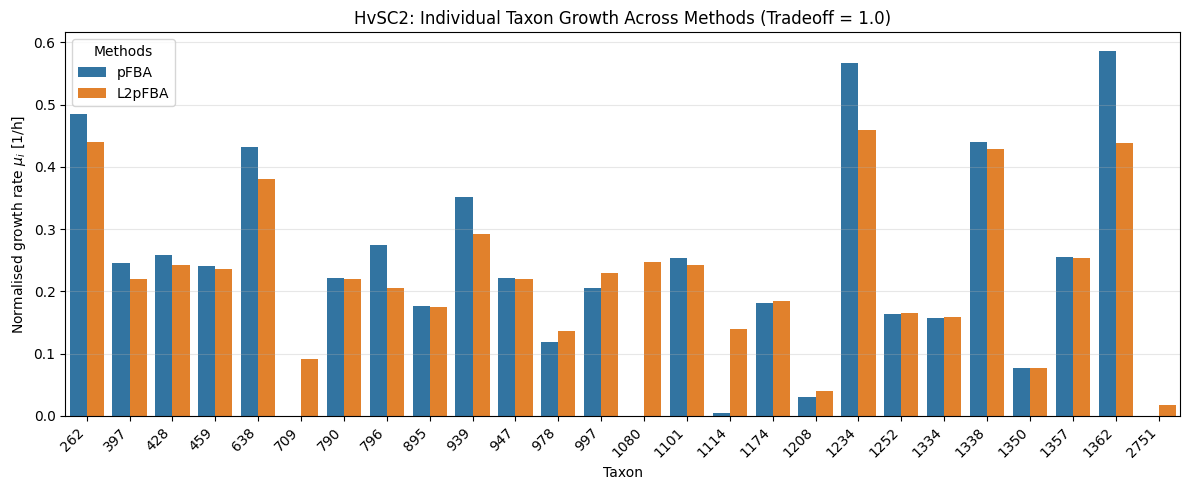
\includegraphics[width=1\linewidth]{fig/HvSC2_individual_growth_methods}
	\caption[Impact of optimisation strategy on individual growth rates of HvSC2]{Impact of optimisation strategy on individual growth rates of HvSC2. Barplot showing scaled $\mu_i$ of HvSC2 at trade-off $\alpha = 1.0$ for different optimisation strategies: pFBA only (blue) and L2-regularisation + pFBA (orange). L2-regularisation yields less extreme growth rates and ensures all strains grow.}
	\label{fig:hvsc2individualgrowthmethods}
\end{figure}


\subsection{Impact of trade-off value $\alpha$ on individual growth rates}
\begin{figure}[H]
	\centering
	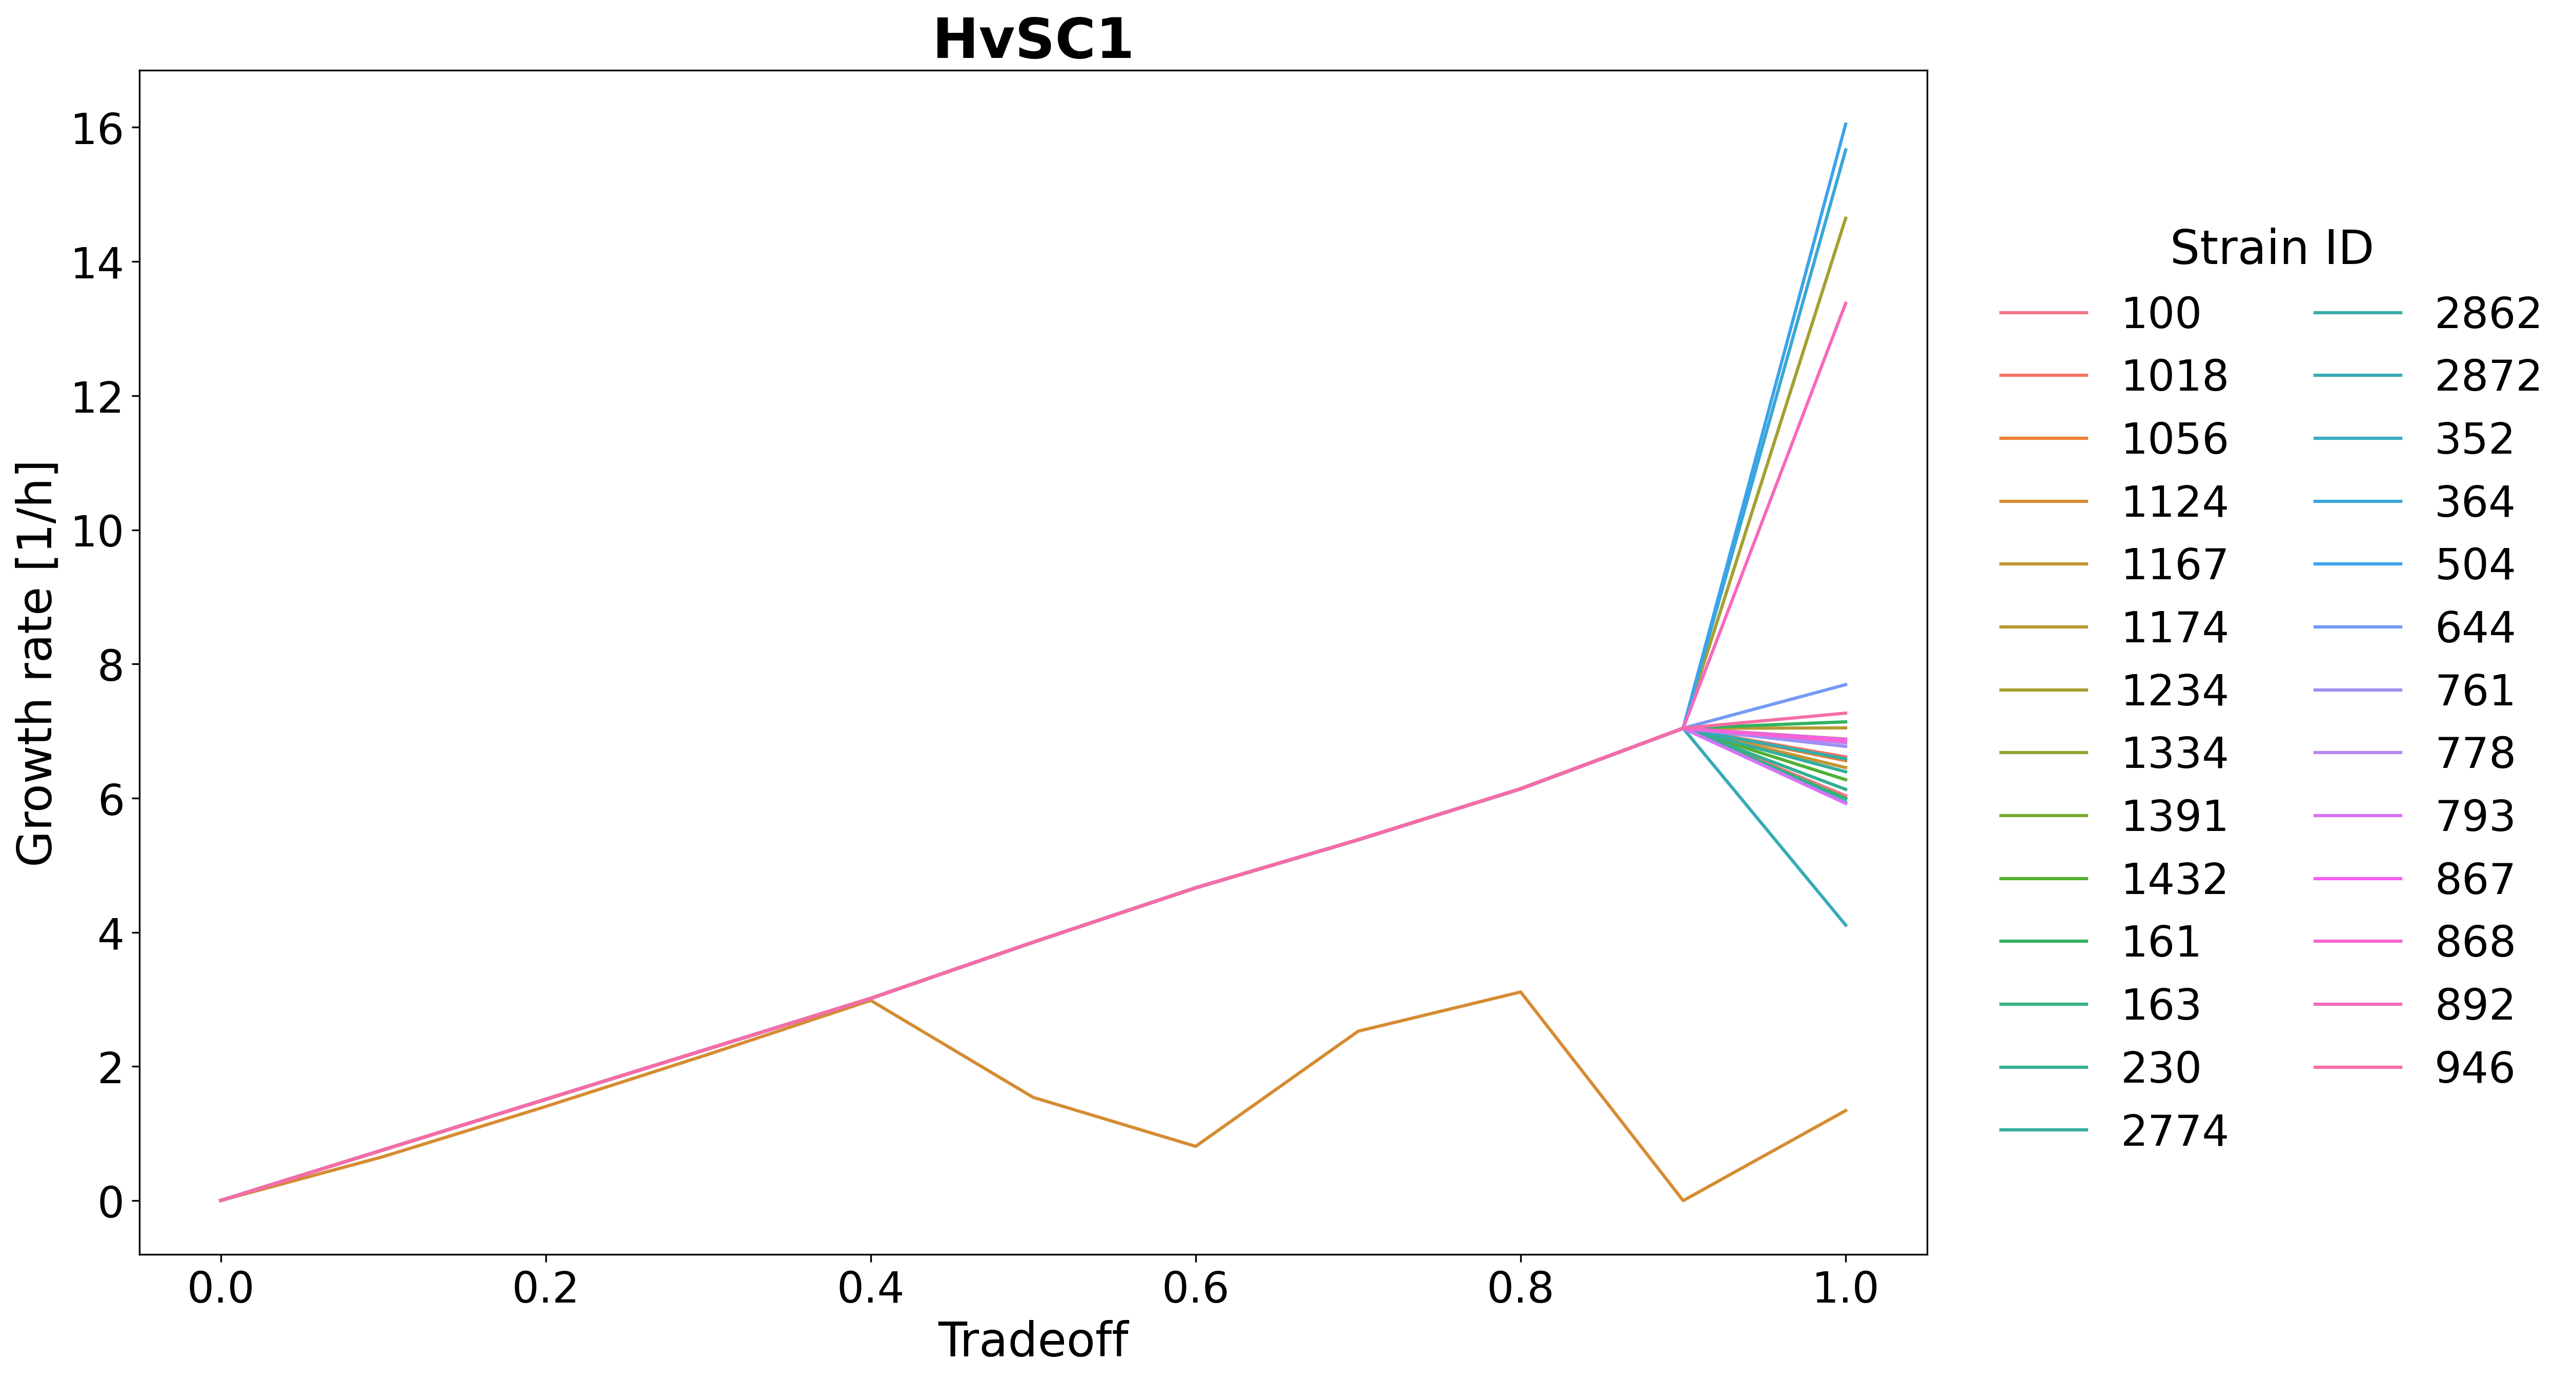
\includegraphics[width=1\linewidth]{fig/HvSC1_individual_growth_tradeoff}
	\caption[Impact of trade-off value $\alpha$ on individual growth rates of HvSC1]{Impact of trade-off value $\alpha$ on individual growth rates of HvSC1. Growth rates of individual community members evaluated at trade-off parameters $\alpha$ between 0.0 and 1.0. Bifurcation of growth rates occurs at $\alpha = 0.96$, strain 1124 diverges at $\alpha = 0.4$. Colour indicates strain ID.}
	\label{fig:hvsc1individualgrowthtradeoff}
\end{figure}

\begin{figure}[H]
	\centering
	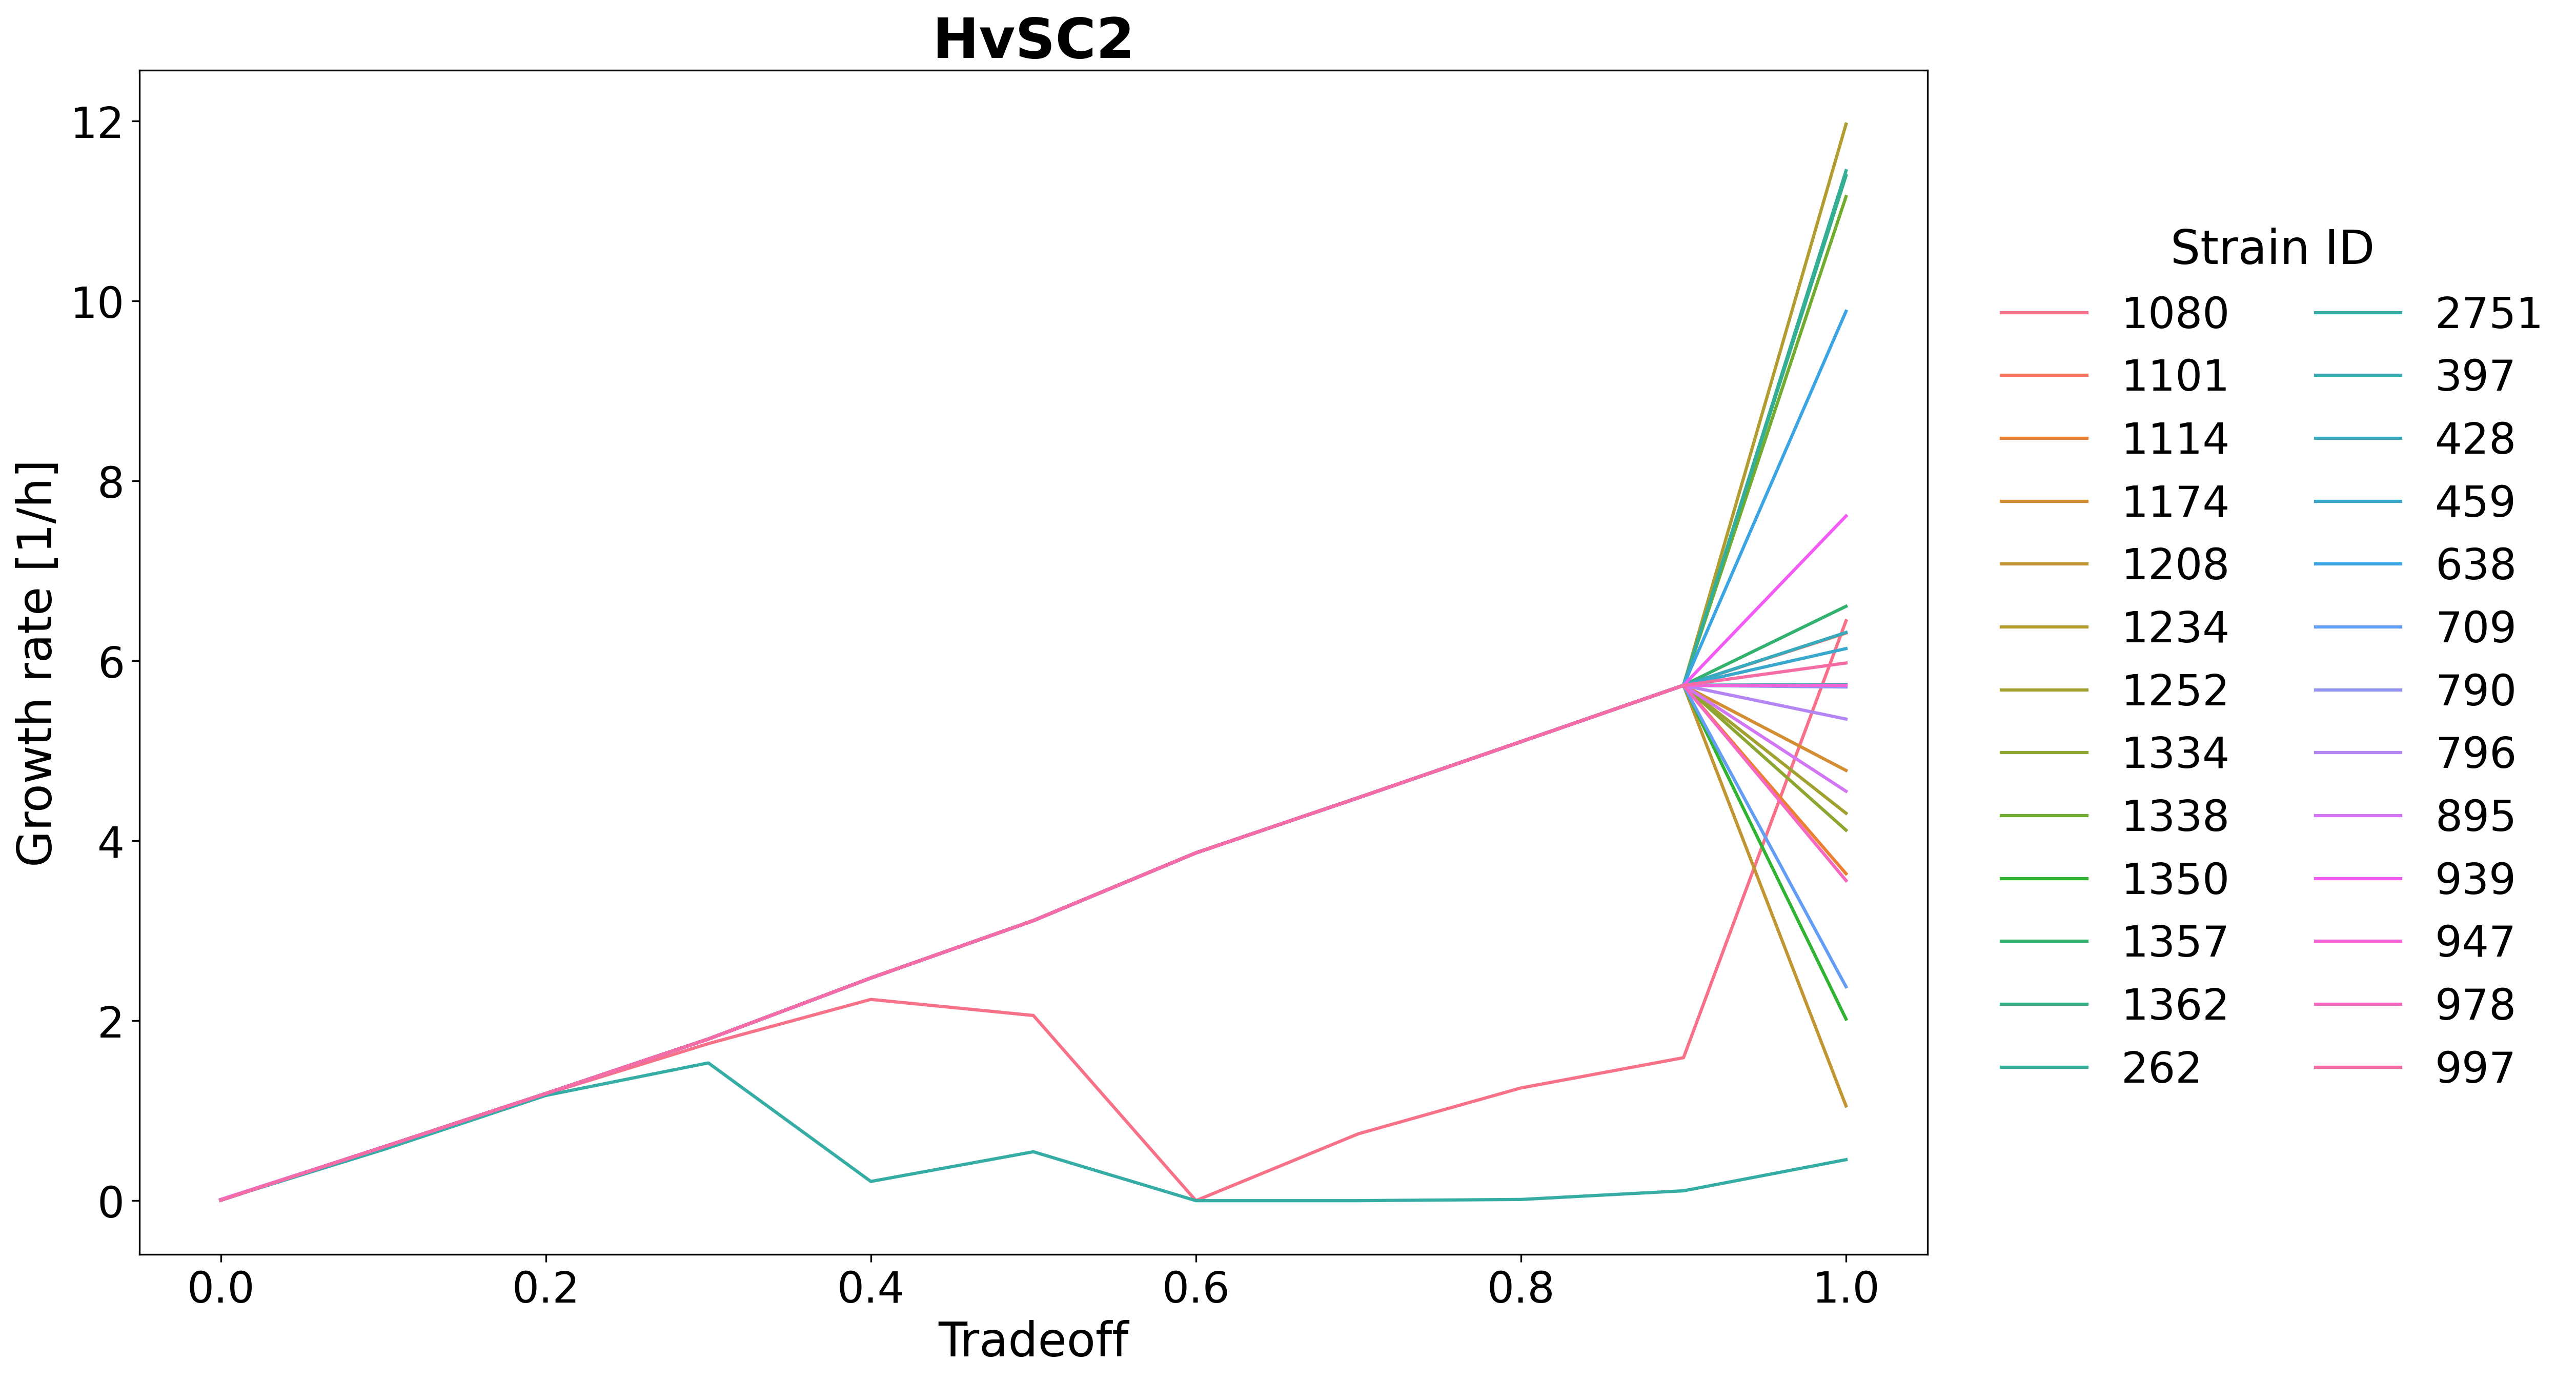
\includegraphics[width=1\linewidth]{fig/HvSC2_individual_growth_tradeoff}
	\caption[Impact of trade-off value $\alpha$ on individual growth rates of HvSC2]{Impact of trade-off value $\alpha$ on individual growth rates of HvSC2. Growth rates of individual community members evaluated at trade-off parameters $\alpha$ between 0.0 and 1.0. Bifurcation of growth rates occurs at $\alpha = 0.96$, with two strains diverging at smaller $\alpha$. Colour indicates strain ID.}
	\label{fig:hvsc2individualgrowthtradeoff}
\end{figure}

\section{Supplementary Tables}

\begin{longtable}{lll}
	\caption{Medium Composition and Exchange Reaction Bounds}
	\label{tab:medium_composition_2}\\
	\toprule
	Compound Name & Exchange Reaction & Upper Uptake Bound \\
	\midrule
	\endfirsthead
	
	\multicolumn{3}{c}%
	{{\tablename\ \thetable{} -- continued from previous page}} \\
	\toprule
	Compound Name & Exchange Reaction & Upper Uptake Bound \\
	\midrule
	\endhead
	
	\midrule
	\multicolumn{3}{r}{{Continued on next page}} \\
	\endfoot
	
	\bottomrule
	\endlastfoot
		(R)-3-Hydroxytetradecanoate & EX\_R\_3httdca\_m & 0.1 \\
		2-Ketogluconate & EX\_2kgnd\_m & 10.0 \\
		4-Aminobutyrate & EX\_4abut\_m & 10.0 \\
		Ammonium & EX\_nh4\_m & 1000.0 \\
		Calcium & EX\_ca2\_m & 1000.0 \\
		Chloride & EX\_cl\_m & 1000.0 \\
		cis-Aconitate & EX\_acon\_C\_m & 0.1 \\
		Citrate & EX\_cit\_m & 10.0 \\
		Cobalt & EX\_cobalt2\_m & 1000.0 \\
		Copper & EX\_cu2\_m & 1000.0 \\
		D-Fructose & EX\_fru\_m & 10.0 \\
		D-Glucose & EX\_glc\_\_D\_m & 10.0 \\
		Diacetylchitobiose & EX\_dachi\_m & 0.1 \\
		Fumarate & EX\_fum\_m & 10.0 \\
		Glycerol & EX\_glyc\_m & 10.0 \\
		Glycine & EX\_gly\_m & 10.0 \\
		Glycyl-L-asparagine & EX\_gly\_asn\_\_L\_m & 10.0 \\
		Glycyl-L-glutamine & EX\_glygln\_m & 10.0 \\
		Iron ($\text{Fe}^{2+}$) & EX\_fe2\_m & 1000.0 \\
		Iron ($\text{Fe}^{3+}$) & EX\_fe3\_m & 1000.0 \\
		L-Alanine & EX\_ala\_\_L\_m & 10.0 \\
		L-Asparagine & EX\_asn\_\_L\_m & 0.1 \\
		L-Aspartate & EX\_asp\_\_L\_m & 10.0 \\
		L-Glutamate & EX\_glu\_\_L\_m & 10.0 \\
		L-Isoleucine & EX\_ile\_\_L\_m & 10.0 \\
		L-Leucine & EX\_leu\_\_L\_m & 10.0 \\
		L-Malate & EX\_mal\_\_L\_m & 10.0 \\
		L-Proline & EX\_pro\_\_L\_m & 0.1 \\
		L-Serine & EX\_ser\_\_L\_m & 10.0 \\
		L-Threonine & EX\_thr\_\_L\_m & 0.1 \\
		L-Tyrosine & EX\_tyr\_\_L\_m & 0.1 \\
		L-Valine & EX\_val\_\_L\_m & 10.0 \\
		Magnesium & EX\_mg2\_m & 1000.0 \\
		Maltose & EX\_malt\_m & 10.0 \\
		Manganese & EX\_mn2\_m & 1000.0 \\
		Molybdate & EX\_mobd\_m & 1000.0 \\
		N-Acetyl-D-glucosamine 1-phosphate & EX\_acgam1p\_m & 0.1 \\
		N-Acetyl-D-mannosamine & EX\_acmana\_m & 0.1 \\
		Nickel & EX\_ni2\_m & 1000.0 \\
		Oxygen & EX\_o2\_m & 1000.0 \\
		Phosphate & EX\_pi\_m & 1000.0 \\
		Potassium & EX\_k\_m & 1000.0 \\
		Proton & EX\_h\_m & 1000.0 \\
		Quinate & EX\_quin\_m & 10.0 \\
		Shikimate & EX\_skm\_m & 0.1 \\
		Sodium & EX\_na1\_m & 1000.0 \\
		Succinate & EX\_succ\_m & 10.0 \\
		Sucrose & EX\_sucr\_m & 0.1 \\
		Sulfate & EX\_so4\_m & 1000.0 \\
		Tyramine & EX\_tym\_m & 10.0 \\
		UDP-N-acetyl-D-glucosamine & EX\_uacgam\_m & 0.1 \\
		Water & EX\_h2o\_m & 1000.0 \\
		Zinc & EX\_zn2\_m & 1000.0 \\
\end{longtable}
	
\begin{longtable}{lllll}
	\caption{Taxonomic classification and Gram stain status of community members}
	\label{tab:syncom_isolates}\\
	\toprule
	Isolate & SynCom & Class & Species & Gram stain \\
	\midrule
	\endfirsthead
	
	\multicolumn{5}{c}%
	{{\tablename\ \thetable{} -- continued from previous page}} \\
	\toprule
	Isolate & SynCom & Class & Species & Gram stain \\
	\midrule
	\endhead
	
	\midrule
	\multicolumn{5}{r}{{Continued on next page}} \\
	\endfoot
	
	\bottomrule
	\endlastfoot
		1174 & Both & Betaproteobacteria & \textit{Hydrogenophaga} sp. BPS33 & negative \\
		1334 & Both & Actinobacteria & \textit{Arthrobacter} sp. FB24 & positive \\
		1234 & Both & Alphaproteobacteria & \textit{Neorhizobium galegae} & negative \\
		892 & HvSC1 & Alphaproteobacteria & \textit{Bosea} sp. F3-2 & negative \\
		2774 & HvSC1 & Chitinophagia & \textit{Paraflavitalea speifideaquilana} & negative \\
		161 & HvSC1 & Betaproteobacteria & \textit{Roseateles chitinivorans} & negative \\
		352 & HvSC1 & Betaproteobacteria & \textit{Polaromonas} sp. JS666 & negative \\
		644 & HvSC1 & Betaproteobacteria & \textit{Acidovorax} sp. A79 & negative \\
		868 & HvSC1 & Betaproteobacteria & \textit{Roseateles} sp. DAIF2 & negative \\
		946 & HvSC1 & Betaproteobacteria & \textit{Variovorax paradoxus} & negative \\
		1018 & HvSC1 & Betaproteobacteria & \textit{Variovorax} sp. WS11 & negative \\
		1056 & HvSC1 & Betaproteobacteria & \textit{Variovorax} sp. KK3 & negative \\
		2862 & HvSC1 & Betaproteobacteria & \textit{Mitsuaria} sp. 7 & negative \\
		100 & HvSC1 & Flavobacteriia & \textit{Flavobacterium soyae} & negative \\
		230 & HvSC1 & Flavobacteriia & \textit{Flavobacterium} sp. MDT1-60 & negative \\
		867 & HvSC1 & Flavobacteriia & \textit{Flavobacterium} sp. RS13.1 & negative \\
		1124 & HvSC1 & Flavobacteriia & \textit{Flavobacterium pectinovorum} & negative \\
		1167 & HvSC1 & Flavobacteriia & \textit{Flavobacterium soyae} & negative \\
		1391 & HvSC1 & Flavobacteriia & \textit{Flavobacterium pectinovorum} & negative \\
		364 & HvSC1 & Gammaproteobacteria & \textit{Stenotrophomonas rhizophila} & negative \\
		2872 & HvSC1 & Actinobacteria & \textit{Nocardioides} sp. B-3 & positive \\
		504 & HvSC1 & Betaproteobacteria & \textit{Pseudoduganella} sp. S-14 & negative \\
		761 & HvSC1 & Betaproteobacteria & \textit{Herbaspirillum hiltneri} & negative \\
		163 & HvSC1 & Gammaproteobacteria & \textit{Pseudomonas} sp. MM213 & negative \\
		793 & HvSC1 & Gammaproteobacteria & \textit{Pseudomonas fluorescens} & negative \\
		778 & HvSC1 & Alphaproteobacteria & \textit{Pararhizobium qamdonense} & negative \\
		1432 & HvSC1 & Alphaproteobacteria & \textit{Shinella zoogloeoides} & negative \\
		709 & HvSC2 & Bacilli & \textit{Bacillus thuringiensis} & positive \\
		2751 & HvSC2 & Bacilli & \textit{Priestia megaterium} & positive \\
		796 & HvSC2 & Alphaproteobacteria & \textit{Caulobacter segnis} & negative \\
		638 & HvSC2 & Actinobacteria & \textit{Cellulomonas} sp. NS3 & positive \\
		1338 & HvSC2 & Chitinophagia & \textit{Chitinophaga filiformis} & negative \\
		428 & HvSC2 & Betaproteobacteria & \textit{Acidovorax} sp. A79 & negative \\
		939 & HvSC2 & Alphaproteobacteria & \textit{Devosia} sp. FJ2-5-3 & negative \\
		1080 & HvSC2 & Alphaproteobacteria & \textit{Devosia rhizoryzae} & negative \\
		262 & HvSC2 & Gammaproteobacteria & \textit{Pseudoxanthomonas} sp. SE1 & negative \\
		1362 & HvSC2 & Gammaproteobacteria & \textit{Lysobacter} sp. S4-A87 & negative \\
		1114 & HvSC2 & Actinobacteria & \textit{Microbacterium} sp. cx-55 & positive \\
		1208 & HvSC2 & Actinobacteria & \textit{Pseudarthrobacter} sp. WHRI 8279 & positive \\
		1350 & HvSC2 & Actinobacteria & \textit{Microbacterium foliorum} & positive \\
		978 & HvSC2 & Actinobacteria & \textit{Nocardioides} sp. W7 & positive \\
		397 & HvSC2 & Gammaproteobacteria & \textit{Pseudomonas chlororaphis} & negative \\
		790 & HvSC2 & Gammaproteobacteria & \textit{Pseudomonas laurylsulfatiphora} & negative \\
		997 & HvSC2 & Gammaproteobacteria & \textit{Pseudomonas} sp. MPB26 & negative \\
		1357 & HvSC2 & Gammaproteobacteria & \textit{Metapseudomonas lalkuanensis} & negative \\
		459 & HvSC2 & Alphaproteobacteria & \textit{Ensifer canadensis} & negative \\
		1101 & HvSC2 & Alphaproteobacteria & \textit{Sinorhizobium} sp. RAC02 & negative \\
		895 & HvSC2 & Alphaproteobacteria & \textit{Sphingomonas hankookensis} & negative \\
		947 & HvSC2 & Alphaproteobacteria & \textit{Sphingomonas} sp. & negative \\
		1252 & HvSC2 & Alphaproteobacteria & \textit{Sphingobium cloacae} & negative \\
\end{longtable}
	
%%%%%%%%%%%%%%%%%%%%%%%%%%%%%%%%%%%%%%%%%%%%%%
%%    End of the main document              %%
%%%%%%%%%%%%%%%%%%%%%%%%%%%%%%%%%%%%%%%%%%%%%%

\backmatter

\printindex

% do not change this file
\begin{otherlanguage}{ngerman}

\chapter*{Ehrenwörtliche Erklärung}

Hiermit versichere ich, Emma Tullius, die vorliegende \thesistypegerman{} selbstständig verfasst und keine anderen als die angegebenen Quellen und Hilfsmittel benutzt zu haben.
Alle Stellen, die aus den Quellen entnommen wurden, sind als solche kenntlich gemacht worden.
Diese Arbeit hat in gleicher oder ähnlicher Form noch keiner Prüfungsbehörde vorgelegen.

\vspace{3cm}

\noindent Düsseldorf, \thesissubmissionday{}. \DTMmonthname{\thesissubmissionmonth} \thesissubmissionyear{} \hfill \makeatletter\@author\makeatother

\end{otherlanguage}
 % Input nicht include, damit es nur eine Seite wird.
\begin{otherlanguage}{ngerman}

\section*{Erklärung zur Nutzung generativer KI}

Im Rahmen der vorliegenden \thesistypegerman{} wurde generative KI zu folgenden Zwecken genutzt:

% Nicht zutreffendes Auskommentieren
% Passend ändern, das hier sind Vorschläge
% Weitere Werkzeuge gegebenenfalls in ähnlichem Stil ergänzen

\begin{itemize}
 \item DeepL Write zur sprachlichen Überarbeitung.
 \item Claude und Gemini zur Unterstützung beim Debugging.
 \item Copilot während der Arbeit am Code als integriertes Werkzeug in der IDE.
\end{itemize}


\end{otherlanguage}

  % Input nicht include, damit es nur eine Seite wird.

\cleardoublepage

\end{document}
